\documentclass[11pt, oneside]{elsarticle}
\usepackage[utf8]{inputenc}
\usepackage{bm}
\usepackage{amsmath}
\usepackage{amsfonts}
\usepackage{amssymb}
\usepackage{graphicx}
\usepackage{xcolor}
\usepackage{cancel}
\usepackage{caption}
\usepackage{subfigure}
\usepackage{algorithm}
\usepackage{algpseudocode}

\subfiglabelskip=0pt

%\newcommand{\codetitlestyle}[1]{\small\textit{#1}\hspace{0.1cm}}
\newcommand{\belowtitleskip}{2pt}%\smallskipamount}
%\newcommand{\captionposition}{t}

%\newcommand{\mmo}[1]{\emph{#1}}

%\renewcommand{\ttdefault}{pcr}
\usepackage[T1]{fontenc}
\usepackage{lmodern}
\usepackage[top=3cm,bottom=4cm,left=3cm,right=3.2cm,asymmetric]{geometry}


\newcommand{\N}[1]{\check{#1}}
\newcommand{\D}[1]{\overline{#1}}


\newcommand{\includecode}[2][py]{\lstinputlisting[caption=#2,label=list:#2,style=pythonstyle,
float=!htpb]{#2}}

\newcommand{\mmo}[1]{({\bf mmo comment:} \emph{#1})}
\bibliographystyle{plain}

\begin{document}
\begin{frontmatter}

\title{Assessment of a Shen-Fourier turbulent channel flow solver for large-scale simulations}
\author[mmo]{Mikael Mortensen}
\ead{mikaem@math.uio.no}
%\date{}							% Activate to display a given date or no date
\address[mmo]{Department of Mathematics, Division of Mechanics, University of Oslo}

\begin{abstract}
A fully (pseudo-)spectral solver for direct numerical simulations of large-scale turbulent channel flows is described. The solver utilizes the Chebyshev base functions suggested by J. Shen [SIAM J. Sci. Comput., 16, 1, 1995], that lead to stable and robust numerics, even at very large scale. New algorithms for direct solution of the linear systems are devised, and we show that the solver is accurate and applicable for very large simulations. Specifically, the solver is shown to reproduce first order statistics of a channel flow at $Re_{\tau}=2000$ by Hoyas and Jim\'{e}nez [Phys. Fluids, 18(1), 2006], which is higher than has been achieved in a channel by a fully spectral method before. 
\end{abstract}
\begin{keyword}
DNS \sep Fourier \sep Chebyshev
\end{keyword}

\end{frontmatter}
\section{Introduction}
Direct Numerical Simulations (DNS) of turbulent flows is a very important research tool, utilized across a range of scientific communities. DNS is used extensively to validate statistical models, and to further our understanding of complex mechanisms taking place inside turbulent flows. One of the many advantages of DNS is that it provides all information about a flow, and quantities that can be very hard to study experimentally, like velocity-pressure interactions, are trivially extracted from a DNS. In this regard, DNS both complements and extends the knowledge we are able to extract from experiments.

The most commonly known DNS use simple geometries, because turbulence physics may then most easily be isolated and studied. Isotropic and homogeneous turbulence are usually studied in triply periodic domains, which allows a spectral Fourier decomposition in all three spatial directions. The equations are solved in spectral space and nonlinearities are usually handled with pseudo-spectral techniques. An important feature is that the pressure can be trivially eliminated, which simplifies the Navier-Stokes equations substantially.

Inhomogeneous, wall bounded, flows, successfully studied with DNS are, e.g., the pipe flow, free shear layers and channel flow between two parallel plates (both Couette and Poiseuille). In this paper we will constrain ourselves to the pressure driven Poiseuille channel flow. In a channel there are two periodic directions that can be handled with Fourier expansions, whereas the wall normal direction is non-periodic and requires a different type of discretization. There are many challenges associated with this inhomogeneity not faced by the pure Fourier solvers, but the first problem at hand is the discretization. The first DNS channel solvers typically used a Chebyshev expansion for the wall-normal direction and, as such, were still able to obtain spectral accuracy in all three spatial directions. A Chebyshev-tau technique, that utilize the recurrence relations of the Chebyshev polynomials, is then used to approximate derivatives, and the coefficient matrices that appear (tridiagonal) can be inverted directly and efficiently. A downside to the Chebyshev-tau method is usually quoted \cite{canuto1988} as numerical stability and roundoff errors, caused by the recurrence relation, and severe condition numbers of the coefficient matrices. For Chebyshev-tau methods the condition numbers have been reported to grow with size as $\mathcal{O}(N^8)$, for a discretization using N points in the wall-normal direction. Discouraged by these numbers, all major recent channel flow simulations have found other, non-spectral, ways of discretizing the non-periodic direction. 


The largest known channel simulations to date have been performed by Lee and Moser \cite{leemoser15}, where for $Re_{\tau}\approx 5200$ they used a computational box of resolution $[10240 \times 1530 \times 7680]$ for the streamwise, wall-normal and spanwise directions, respectively. Lee and Moser used seventh-order B-splines for the wall-normal direction. Other simulations of similar magnitude are performed by Hoyas and Jim\'{e}nez \cite{hoyas06, hoyas08}, Lozano-Duran and Jim\'{e}nez \cite{Lozano2014} and Bernardini, Pirozzoli and Orlandi \cite{bernardini2014}. Bernardini et al. used second order finite differences throughout. The Jim\'{e}nez group used dealiased Fourier in the two periodic directions and seventh order compact finite differences, with fourth-order consistency and extended spectral-like resolution \cite{Lele92}, for the wall-normal direction. The solver by Jim\'{e}nez' group is reported to switch from Chebyshev to finite differences if the resolution is above a certain threshold \cite{hoyas08} (reached around $Re_{\tau}=1000$). In other words, they attempt to use spectral methods for as large $Re_{\tau}$ as possible. Spectral methods are attractive for their accuracy, but also for their resolution properties, that are superior to those of any finite difference or spline method. As such, it is desirable to develop fully spectral solvers that can be used for large-scale turbulence simulations.

In his seminal papers \cite{Shen94,Shen95}, Jie Shen describe how to make Legendre and Chebyshev basis functions that lead to sparse matrices, susceptible to fast ($\mathcal{O}(N)$) direct solvers. To the authors knowledge, the bases have not been used for large-scale channel flow simulations, and algorithms for the required direct solvers have not, until now, been devised. Shen's bases have been used for the Navier Stokes equations before, though. Bouchon et.al.  \cite{Bouchon01} describe a spectral-Galerkin formulation very similar to the one used in this paper. However, they choose the Legendre basis over the Chebyshev, due to the simpler structure of the matrices and the lack of weight functions for the Legendre basis. Also, the channel simulations performed were rather small, and there is also the issue of fast transforms for the Legendre basis.

In this paper we will describe and assess a channel flow solver based on Shen's Chebyshev basis \cite{Shen95}. We will give a proper description of the theoretical basis in Sec~\ref{sec:prelim}, the discretization of Navier-Stokes equations in Sec~\ref{sec:discretizationNS} and we will here describe necessary algorithms, including a new fast direct solver for the biharmonic problem that arise in Sec~\ref{sec:implementation}. We will finally show in Sec~\ref{sec:verification} that roundoff is not a major issue, and that the spectral-Galerkin method is in deed applicable to large-scale simulations, larger than what has been achieved for fully spectral channel simulations before.

\section{Preliminaries}
\label{sec:prelim}
The Navier-Stokes equations used to describe turbulent flow in a doubly 
periodic channel can be written in rotational form as
\begin{align}
 \frac{\partial \bm{u}}{\partial t}   &= \bm{\mathcal{H}} + \nu 
 \nabla^2 \bm{u} - \nabla{P}, \notag \\
 \nabla \cdot \bm{u} &= 0, \label{eq:NS}
\end{align}
where $\bm{u}(\bm{x}, t)=(u, v, w)$ is the velocity vector, $\bm{x}=(x, y, z)$ 
and $t$ are position and time and $\bm{\mathcal{H}}(\bm{x}, t) = \bm{u}\times 
\bm{\omega}$, where $\bm{\omega} = \nabla \times \bm{u}$, represents 
the nonlinearity.  The constant dynamic viscosity is denoted as $\nu$ 
and $P(\bm{x}, t)$ is a pressure modified to account for both the driving force, $\beta(t)$, and the kinetic energy, i.e., $P = p + \bm{u} \cdot \bm{u}/2 + \beta y$, where $p$ is the instantaneous 
pressure normalized by a constant density. The computational domain is 
$\Omega=[-1, 1]\times [0, L_y] \times [0, L_z]$ with channel walls 
located at $x=\pm 1$, such that no-slip applies at 
$ \bm{u}(\pm 1, y, z, t) = 0$. The walls are spanning 
the $y-z$ plane and the equations are periodic in the $y$ and $z$ directions with periodic lengths $L_y$ and $L_z$, respectively.

The Navier Stokes equations are discretized using Fourier basis functions for the periodic directions, and a combination of Chebyshev polynomials in the wall normal direction. Three different sets of basis functions and function spaces are relevant for the wall normal direction
\begin{align}
&  \phi_k(x) = T_k(x), & V_{N_x} &= \text{span}\{\phi_k\}_{k=0}^{N_x} \label{eq:Tk}\\
& \D{\phi}_k(x) = T_k(x) - T_{k+2}(x), & \D{V}_{N_x} &= \text{span} \{ \D{\phi}_k\}_{k=0}^{N_x-2} \label{eq:phiD}\\
& \N{\phi}_k(x) = T_k(x) - \frac{2(k+2)}{k+3} T_{k+2}(x) + 
\frac{k+1}{k+3} T_{k+4}, & \N{V}_{N_x} &= \text{span} \{\N{\phi}_k\}_{k=0}^{N_x-4} \label{eq:phiN} 
\end{align}
where $T_k(x)$ is the $k$'th degree Chebyshev polynomial of the first kind. The 
basis functions and function spaces in (\ref{eq:phiD}) and (\ref{eq:phiN}) were 
suggested by Shen, and satisfy, respectively, the boundary conditions 
$\D{\phi}_k(\pm 1) = 0$, $\N{\phi}_k(\pm 1)=0$ and $\N{\phi}'_k(\pm 1)=0$. The 
last two function spaces may alternatively be written as $\D{V}_{N_x} = \{v \in 
V_{N_x}: v(\pm 1)=0 \}$ and $\N{V}_{N_x} = \{v \in V_{N_x}: v(\pm 1) = v'(\pm 
1) = 0 \}$.  

Three-dimensional basis functions and function spaces, that are periodic in $y$ 
and $z$ directions, can now be defined as
\begin{align}
  \psi_{\bm{k}}(\bm{x}) = \phi_{l}(x)e^{ \imath(\underline{m} y + \underline{n} z)}, \quad V_N &= \text{span} \{ \psi_{\bm{k}}(\bm{x}):\, \bm{k} \in K_N  \}, \\
  \D{\psi}_{\bm{k}}(\bm{x}) = \D{\phi}_{l}(x)e^{ \imath(\underline{m} y + \underline{n} z)}, \quad \D{V}_N &= \text{span} \{ \D{\psi}_{\bm{k}}(\bm{x}):\, \bm{k} \in \D{K}_N  \}, \\
  \N{\psi}_{\bm{k}}(\bm{x}) = \N{\phi}_{l}(x)e^{ \imath(\underline{m} y + \underline{n} z)}, \quad \N{V}_N &= \text{span} \{ \N{\psi}_{\bm{k}}(\bm{x}):\, \bm{k} \in \N{K}_N  \},
\end{align}
where $\imath=\sqrt{-1}$ and 
\begin{align}
K_N = \Big\{\bm{k} \in \mathcal{Z}\times\mathcal{R}^2 / &(l, \underline{m}, \underline{n}) \in \left( l, \frac{2 \pi m}{L_y}, \frac{2 \pi n}{L_z} \right), \text{where} \notag \\
 &(l, m, n) \in  [0, \ldots, N_x] \times [-\frac{N_y}{2},\ldots, 
 \frac{N_y}{2}-1] \times[-\frac{N_z}{2},\ldots, \frac{N_z}{2}-1] \Big\} 
 \label{eq:wavenumbermesh}
\end{align}
is the wavenumber mesh for $V_N$. The other two wavenumber meshes $\D{K}_N$ and 
$\N{K}_N$ are both equal to $K_N$ except from in index $l$ that 
ranges $[0, 1, \ldots, N_x-2]$ and $[0, 1, \ldots, N_x-4]$ for $\D{K}_N$ 
and $\N{K}_N$ respectively, see (\ref{eq:phiD}) and (\ref{eq:phiN}). We use 
notation $K^p(m, n)=K_N(0, m, n)$ when referring to only the two periodic 
dimensions of $K_N$. Likewise, ${K}^x(l)={K}_N(l, 0, 0), \D{K}^x(l)=\D{K}_N(l, 0, 0)$ and $\N{K}^x(l)=\N{K}_N(l, 0, 0)$ refer to the wavenumbers in the wall normal direction.

The computational mesh in real space can be created using $N = (N_x, N_y, 
N_z)$ intervals, where the two periodic directions use uniform intervals. The 
computational mesh is given as
\begin{align}
  X_N = \Big\{ \bm{x} \in \mathcal{R}^3/&(x_i, y_j, z_k) \in \left( h(i), \frac{jL_y}{N_y}, \frac{kL_z}{N_z} \right), \text{where} \notag \\
  &(i, j, k) \in [0, 1, \ldots, N_x] \times [0, 1, \ldots, N_y-1] \times [0, 1, \ldots, N_z-1] \Big\} \label{eq:Xn}
\end{align}
where $x_i = h(i)$ represents either Gauss-Lobatto or Gauss-Chebyshev points
\begin{equation}
 h(i) = \begin{cases}
   \cos \left(\frac{i \pi }{N_x} \right) \, &\forall \, i=0,1, \ldots, N_x \quad  \text{for Gauss-Lobatto points}, \\
   \cos \left(\frac{(2i +1)\pi}{2N_x+2} \right) \, &\forall \, i=0,1, \ldots, N_x \quad  \text{for Gauss-Chebyshev points}. \\
 \end{cases}
\end{equation}

For the Navier Stokes equations we look for solutions of the velocity 
components of the form
\begin{align}
u(\bm{x}, t) &= \frac{1}{N_yN_z}\sum_{\bm{k} \in \N{K}_N} \hat{u}_{\bm{k}}(t) 
\N{\psi}_{\bm{k}}(\bm{x}), \label{eq:u_solx} \\
v(\bm{x}, t) &= \frac{1}{N_yN_z}\sum_{\bm{k} \in \D{K}_N} \hat{v}_{\bm{k}}(t) 
\D{\psi}_{\bm{k}}(\bm{x}), \label{eq:u_soly} \\
w(\bm{x}, t) &= \frac{1}{N_yN_z}\sum_{\bm{k} \in \D{K}_N} \hat{w}_{\bm{k}}(t) 
\D{\psi}_{\bm{k}}(\bm{x}), \label{eq:u_solz}
\end{align}
where $\hat{u}_{\bm{k}}(t) = \hat{u}(l, {m}, {n}, t)$ are the expansion 
coefficients for the velocity component in $x$-direction (and similar for the 
other two components) and the scaling by $N_y$ and $N_z$ is merely for 
convenience 
and compliance with the definition used for the inverse discrete Fourier 
transform. Note that from now on we will simply use the notation $\hat{u}$ for 
$\hat{u}_{\bm{k}}(t)$, when it is possible to simplify without loss of clarity. 
Likewise we will simply use $u$ for $u(\bm{x}, t)$. 

If the expansion coefficients $\hat{u}$  are known for the entire wavenumber 
mesh (\ref{eq:wavenumbermesh}), then the expression (\ref{eq:u_solx}) may be 
evaluated on the mesh (\ref{eq:Xn}) using fast Fourier and fast Shen inverse 
transforms as
\begin{align}
u(x_i, y_j, z_k, t) &= \underbrace{\frac{1}{N_z}\sum_n 
\underbrace{\frac{1}{N_y} \sum_m \underbrace{\sum_l 
\hat{u}(l,m,n,t)\N{\phi}_l(x_i)}_{\N{\mathcal{S}}_x^{-1}} e^{\imath 
\underline{m} 
y_j}}_{\mathcal{F}_y^{-1}} e^{\imath \underline{n} z_k}}_{\mathcal{F}_z^{-1}} , 
\quad \forall \, \bm{x} \in X_N, \notag \\
  u &= \N{\mathcal{T}}^{-1}(\hat{u}) =  \mathcal{F}^{-1}_z (\mathcal{F}^{-1}_y 
  (\N{\mathcal{S}}^{-1}_x (\hat{u}))), \quad \forall \, \bm{x} \in X_N.  
  \label{eq:ifft} 
\end{align}
Here $\N{\mathcal{T}}^{-1}$ is used as short notation for the complete inverse 
transform, $\mathcal{F}_{y}^{-1}$ and $\mathcal{F}_{z}^{-1}$ represent inverse 
Fourier transforms along directions $y$ and $z$ respectively, and the inverse 
Shen transform $\N{\mathcal{S}}_{x}^{-1}$ is performed along the wall normal 
$x$ direction. Note that the transforms are applied sequentially to the entire 
computational mesh. The inverse Shen transform may be computed using fast 
Chebyshev transforms for all the three bases in (\ref{eq:Tk}, \ref{eq:phiD}, 
\ref{eq:phiN}). The inverse transforms are slightly different for the three 
bases and 
${\mathcal{S}}^{-1}, \D{\mathcal{S}}^{-1}$ and $\N{\mathcal{S}}^{-1}$ are used 
to distinguish between them with obvious notation. 

A three-dimensional scalar product in the weighted $L^2_w(\Omega)$ space is defined as
\begin{align}
 \left<u, v\right>_w &= \int_{\Omega} {u(\bm{x}) v^*(\bm{x})}w\,dxdydz, 
\end{align}
where $v^*$ is the comlex conjugate of $v$ and the weights $w$ are unity for 
periodic directions and  $w=1/\sqrt{1-x^2}$ for the inhomogeneous direction. In 
this work we will make use of the discrete weighted $l^2_w(\Omega)$ space, 
where quadrature is employed for integration. As such the scalar product 
corresponds to sums that may be computed using fast transforms. Using 
$\N{\psi}_{\bm{k}}$ for $v$ we obtain
\begin{align}
 \left< u, \N{\psi}_{\bm{k}} \right>_w &= h \underbrace{\sum_i 
 \underbrace{\sum_j \underbrace{\sum_k u(x_i, y_j, z_k, t)  e^{-\imath 
 \underline{n} z_k}}_{\mathcal{F}_n}  e^{-\imath \underline{m} y_j} 
 }_{\mathcal{F}_m} \N{\phi}_{l}(x_i) w_i}_{\N{\mathcal{S}}_l},   \notag \\
  &=  h \N{\mathcal{S}}(u) = h \N{\mathcal{S}}_{l} (\mathcal{F}_{{m}} 
  (\mathcal{F}_{{n}}(u))), \quad \forall \, \bm{k} \in \N{K}_N. \label{eq:sst1}
\end{align}
Here $h\N{\mathcal{S}}$ denotes the complete three-dimensional scalar product 
and $h = L_yL_zN_y^{-1}N_z^{-1}$ is a constant. $\mathcal{F}_{{n}}$ and 
$\mathcal{F}_{{m}}$ represent discrete Fourier transforms in $z$- and 
$y$-directions, respectively, and $\N{\mathcal{S}}_{l}(\cdot) = (\cdot, 
\N{\phi}_l)_w$ is used to represent the Shen scalar product in the 
$x$-direction. The weights, $w_i$, required for the Shen transforms are 
defined as
\begin{equation}
 w_i = \begin{cases}
       \frac{\pi}{c_i N_x} &\forall \, i=0,1,\ldots, N_x \quad  \text{for 
       Gauss-Lobatto points},\\
       \frac{\pi}{N_x+1} &\forall \, i=0,1,\ldots, N_x  \quad \text{for 
       Gauss-Chebyshev points},      
 \end{cases}
\end{equation}
where $c_0 = c_{N_x} = 2$ and $c_i = 1$ for $0 < i < N_x$.\footnote{Note that 
$c_{N_x}=1$ for the continuous scalar product $L^2_w(\Omega)$ (see, e.g., Eq. 
(2.7) of \cite{Shen95}), but for the discrete $l^2_w(\Omega)$ it follows that 
$c_{N_x}=2$ due to inexact quadrature for the highest wavenumber.}

The scalar product  $h\N{\mathcal{S}}$ in (\ref{eq:sst1}) does not represent a 
complete transform. To find a transformation between physical $u$ and spectral 
$\hat{u}$ we make use of Eq. (\ref{eq:u_solx}) directly in the first line of (\ref{eq:sst1}) and use extensively the discrete 
orthogonality of the Fourier basis functions
\begin{align}
%\left<u, \N{\psi}_{\bm{k}}\right>_w &= \frac{1}{N_yN_z}\left< 
%\sum_{\bm{m}=(q,r,s) \in \N{K}_N} \hat{u}_{\bm{m}} \N{\psi}_{\bm{m}}, 
%\N{\psi}_{\bm{k}} \right>_w, \notag \\
\left<u, \N{\psi}_{\bm{k}}\right>_w &= \frac{1}{N_yN_z}\left< 
\sum_{(q,r,s) \in \N{K}_N} \hat{u}(q,r,s,t) \N{\psi}(q,r,s), 
\N{\psi}(l,m,n) \right>_w, \notag \\
           &= h \sum_{q=0}^{N_x-4} \sum_{i=0}^{N_x} \N{\phi}_{q}(x_i) 
           \N{\phi}_{l}(x_i) w_i \, \hat{u}(q, {m}, {n}, t), \notag \\
           &= h \sum_{q=0}^{N_x-4} \N{B}_{lq} \hat{u}(q, {m}, {n}, t). 
           \label{eq:sst2}
\end{align}
Here $\{\N{B}_{lq}\}_{l,q=0}^{N_x-4} = (\N{\phi}_q, \N{\phi}_l)_w = 
\sum_{i=0}^{N_x} \N{\phi}_{q}(x_i) \N{\phi}_{l}(x_i) w_i$ is a 
pentadiagonal mass matrix. The complete transformation is now obtained by 
setting Eq. (\ref{eq:sst2}) equal to (\ref{eq:sst1}) and solving for $\hat{u}$. 
Moving to matrix notation we get
\begin{align}
h\sum_{q=0}^{N_x-4} \N{B}_{lq}\, \hat{u}(q, {m}, {n}, t) &= 
h\N{\mathcal{S}}(u)(l, m, n, t), \notag \\
 \hat{u} &= \N{\mathcal{T}}(u) =  \N{B}^{-1}\N{\mathcal{S}}(u), 
 \quad \forall \, \bm{k} \in \N{K}_N, \label{eq:fstB}
\end{align}
where $\N{\mathcal{T}}(u)$ denotes the complete transformation, such that $u = 
\N{\mathcal{T}}^{-1}(\N{\mathcal{T}}(u))$. Note that, since $\N{B}$ assembles to 
a pentadiagonal matrix, the solution ($\N{B}^{-1}$) can be obtained very fast and the complete 
transformation thus requires a fast Chebyshev transform ($\mathcal{O}(N_x \log N_x)$) and 
a fast linear algebraic solve ($\mathcal{O}(N_x)$). Similar transforms $\mathcal{T}$ 
and $\D{\mathcal{T}}$ are defined for the two other bases (\ref{eq:Tk}) and 
(\ref{eq:phiD}), using mass matrices $B_{lq}=(T_q, T_l)_w$ (diagonal) and 
$\D{B}_{lq}=(\D{\phi}_l, \D{\phi}_q)_w$ (tridiagonal) and scalar products 
$\mathcal{S}_l(\cdot) = (\cdot, T_l)_w$ and $\D{\mathcal{S}}_l(\cdot) = (\cdot, 
\D{\phi}_l)_w$. See the Appendix for algorithms for all required transforms.

\section{Discretization of Navier Stokes equations}
\label{sec:discretizationNS}
The Navier Stokes equations (\ref{eq:NS}) are solved using a scheme 
proposed by Kim, Moin and Moser (1987). This scheme is developed by taking the 
Laplacian of the wall normal momentum equation and the curl of the momentum 
equation. Following elimination of the pressure, the equations to solve are 
\begin{align}
\frac{\partial}{\partial t} \nabla^2 u &= h_u + \nu \nabla^4 u, 
\label{eq:biharmonic} \\
\frac{\partial g}{\partial t} &= h_g + \nu \nabla^2 g, \label{eq:g} \\
f + \frac{\partial u}{\partial x} &= 0, \label{eq:f}
\end{align}
where
\begin{align}
f &= \frac{\partial v}{\partial y} + \frac{\partial w}{\partial z}, \\
g &= \frac{\partial w}{\partial y} - \frac{\partial v}{\partial z}, \\
h_u = -\frac{\partial}{\partial x} &\left( \frac{\partial 
\mathcal{H}_y}{\partial y} + \frac{\partial \mathcal{H}_z}{\partial z} \right) 
+ \left(\frac{\partial^2}{\partial y^2} + \frac{\partial^2}{\partial z^2} 
\right) \mathcal{H}_x ,
\\
h_g &= \frac{\partial \mathcal{H}_z}{\partial y} - \frac{\partial 
\mathcal{H}_y}{\partial z}.
\end{align}
The two remaining velocity components are computed from the definitions of $f$ 
and $g$. The biharmonic equation (\ref{eq:biharmonic}) is solved with boundary 
conditions $u(\pm 1) = u'(\pm 1) = 0$, where the Neumann conditions follow 
from the continuity equation. The boundary conditions for Eq. (\ref{eq:g}) are 
$g(\pm 1) = 0$. The variational formulation becomes: Find ${u} \in 
\N{V}_N$, ${g} \in \D{V}_N$ and ${f} \in \D{V}_N$ such that
\begin{align}
	\frac{\partial }{\partial t} \left< \nabla^2 u, \N{\psi}\right>_w &= 
	\left<h_u, \N{\psi} \right>_w + \nu \left<\nabla^4u, \N{\psi}\right>_w 
	&\forall \,\N{\psi} \in \N{V}_N, \label{eq:u1} \\
	\frac{\partial}{\partial t}\left<g, \D{\psi}\right>_w &= \left<h_g, 
	\D{\psi}\right>_w + \nu 
	\left<\nabla^2 g, \D{\psi}\right>_w &\forall \, \D{\psi} \in \D{V}_N ,
	\label{eq:g1} \\
	\left<f, \D{\psi}\right>_w &= \left<\frac{\partial u}{\partial x}, 
	\D{\psi}\right>_w &\forall \, \D{\psi} \in \D{V}_N. \label{eq:f1}
\end{align}
The two remaining velocity components are computed by projection to the 
Dirichlet space $\D{V}_N$: Find 
${v} \in \D{V}_N$ and $w \in \D{V}_N$ such that
\begin{align}
\left<f, \D{\psi}\right>_w &= \left<\frac{\partial v}{\partial y} + 
\frac{\partial w}{\partial z}, \D{\psi}\right>_w \, &\forall \, \D{\psi} \in 
\D{V}_N, \label{eq:f2} \\
\left<g, \D{\psi}\right>_w &= \left<\frac{\partial w}{\partial y}  - 
\frac{\partial v}{\partial z}, \D{\psi}\right>_w \, &\forall \, \D{\psi} \in 
\D{V}_N, \label{eq:g2}
\end{align}
which simplifies considerably because all the derivatives are in periodic 
directions. Written in spectral space Eqs. (\ref{eq:f2}) and (\ref{eq:g2}) 
become simply
\begin{align}
\hat{f}_{\bm{k}} &= \imath \underline{m}\, \hat{v}_{\bm{k}} + \imath 
\underline{n}\, \hat{w}_{\bm{k}} &\forall \, \bm{k} \in \D{K}_N^0, \label{eq:f3} \\
\hat{g}_{\bm{k}} &= \imath \underline{m}\, \hat{w}_{\bm{k}} - \imath 
\underline{n}\, \hat{v}_{\bm{k}} & \forall \, \bm{k} \in \D{K}_N^0, \label{eq:g3}
\end{align}
where $\D{K}_N^0$ is used to denote that these equations can be solved for all 
wavenumbers except $m=n=0$. For $m=n=0$ we solve instead the 
corresponding transformed momentum equations in $y$ and $z$ directions:
\begin{align}
\frac{\partial }{\partial t} \D{B}_{lq}\hat{v}(q, 0, 0, t) &= 
\D{B}_{lq}\hat{\mathcal{H}}_y(q, 0, 0, t) + \nu \D{A}_{lq} \hat{v}(q, 0, 0, t) - \left(\beta(t), \D{\phi}_l \right)_w
& \forall\, l \in \D{K}^x, \label{eq:v0}\\
\frac{\partial }{\partial t} \D{B}_{lq}\hat{w}(q, 0, 0, t) &= 
\D{B}_{lq}\hat{\mathcal{H}}_z(q, 0, 0, t) + \nu \D{A}_{lq} \hat{w}(q, 0, 0, t) 
& \forall\, l \in \D{K}^x,\label{eq:w0}
\end{align}
where $\D{B}_{lq} = \left(\D{\phi}_q, \D{\phi}_l \right)_w$ and $\D{A}_{lq}=\left(\D{\phi}_q^{''}, \D{\phi}_l \right)_w$. Note that (\ref{eq:v0}) is the only place where the driving force, or the mean pressure gradient, $\beta$, enters, and, since it is constant in space, the term $\left(\beta(t), \D{\phi}_l \right)_w$ will only be non-zero for $l=0$.

Equations (\ref{eq:u1}-\ref{eq:f1}) need to be rewritten in terms of one-dimensional scalar products. 
Inserting the expansion (\ref{eq:u_solx}) for $u$ and a similar expansion for $g$ in $\D{V}_N$, the inner products required to solve Eqs. (\ref{eq:u1}-\ref{eq:f1}) are
\begin{align}
\left<\nabla^4u, \N{\psi}_{\bm{k}}\right>_w &= h\left[ \left( 
\N{\phi}_q^{''''}, 
\N{\phi}_l\right)_w -2(\underline{m}^2+\underline{n}^2) \left( \N{\phi}_q^{''}, 
\N{\phi}_l\right)_w + (\underline{m}^2+\underline{n}^2)^2\left( \N{\phi}_q, 
\N{\phi}_l\right)_w  \right] \hat{u}_q, \\
\left< \nabla^2 u, \N{\psi}_{\bm{k}}\right>_w &= h\left[\left( \N{\phi}_q^{''}, 
\N{\phi}_l\right)_w - (\underline{m}^2+\underline{n}^2)\left( \N{\phi}_q, 
\N{\phi}_l \right)_w \right] \hat{u}_q, \\
\left< \nabla^2 g, \D{\psi}_{\bm{k}}\right>_w &= h\left[\left( \D{\phi}_q^{''}, 
\D{\phi}_l\right)_w - (\underline{m}^2+\underline{n}^2)\left( \D{\phi}_q, 
\D{\phi}_l \right)_w \right] \hat{g}_q, \\
\left<\frac{\partial u}{\partial x}, \D{\psi}_{\bm{k}}\right>_w &=
h\left(\N{\phi}_q^{'}, \D{\phi}_l\right)_w \hat{u}_q, \\
\left<h_u, \N{\psi}_{\bm{k}} \right>_w &= 
h\left[-(\underline{m}^2+\underline{n}^2) 
\left(\D{\phi}_q, 
\N{\phi}_l \right)_w \hat{\mathcal{H}}_{x, q} - \imath \underline{m}\left(\D{\phi}_q^{'}, 
\N{\phi}_l \right)_w \hat{\mathcal{H}}_{y, q} - \imath 
\underline{n}\left(\D{\phi}_q^{'}, \N{\phi}_l \right)_w 
\hat{\mathcal{H}}_{z, q}\right], \label{eq:S_hv}
\\
\left< h_g, \D{\psi}_{\bm{k}} \right>_w &= h\left[ \imath \underline{m}\, \left(\D{\phi}_q, \D{\phi}_l \right)_w 
\hat{\mathcal{H}}_{z, q} - \imath \underline{n}\, \left(\D{\phi}_q, \D{\phi}_l \right)_w \hat{\mathcal{H}}_{y, q} 
\right],\label{eq:S_hg}
\end{align}
where for brevity in notation (as before) it is understood that the matrices 
act along the first dimension of the transformed variables, i.e.,  $ 
\left(\N{\phi}_q^{'}, \D{\phi}_l\right)_w \hat{u}_q$ is short for the matrix 
vector product $ \sum_{q=0}^{N_x-4}\left( \N{\phi}_q^{'}, \D{\phi}_l\right)_w 
\hat{u}(q, {m}, {n}, t)$, where $m$ and $n$ are given. The inner products are used to set up linear systems 
of equations for the inhomogeneous wall normal direction. All inner products 
$\left(\cdot, \cdot\right)_w$ can be represented by sparse matrices.
%\begin{align}
%\frac{\partial }{\partial t} \left( \N{\psi}_j^{''}, \N{\psi}_k\right)_w 
%\hat{u}_j &=  \left(h_u, \N{\psi}_k \right)_w + \nu \left(\N{\psi}^{''''}_j, 
%\N{\psi}_k\right)_w \hat{u}_j, \, &\forall \N{\psi}_k \in \N{V}_N, \\
%\frac{\partial}{\partial t}\left(\D{\psi}_j, \D{\psi}_k\right)_w \hat{g}_j &= 
%\left(h_g, \D{\psi}_k\right)_w + \nu \left(\D{\psi}_j^{''}, 
%\D{\psi}_k\right)_w 
%\hat{g}_j, \, &\forall \D{\psi}_k \in \D{V}_N \\
%\left(\D{\psi}_j, \D{\psi}_k\right)_w \hat{f}_j &= \left(\N{\psi}_j^{'}, 
%\D{\psi}_k\right)_w \hat{u}_j, \, &\forall \D{\psi}_k \in \D{V}_N.
%\end{align}
The required matrices $ \N{B}_{lq} = \left( \N{\phi}_q, 
\N{\phi}_l\right)_w, \D{B}_{lq} = \left( \D{\phi}_q, 
\D{\phi}_l\right)_w, \N{A}_{lq} = \left( \N{\phi}_q^{''}, 
\N{\phi}_l\right)_w, 
\D{A}_{lq} = \left( \D{\phi}_q^{''}, \D{\phi}_l\right)_w 
, \D{C}_{lq} = \left(\N{\phi}_q^{'}, \D{\phi}_l\right)_w$ and 
$ \N{C}_{lq} = \left(\D{\phi}_q^{'}, \N{\phi}_l\right)_w$ are given in Table~\ref{tab:matrices}, whereas the matrix $\N{Q}_{lq} = \left(\N{\phi}^{''''}_q, \N{\phi}_l\right)_w$ is given below in Eqs (\ref{eq:N_Q})-(\ref{eq:rk}). 

The convection vector $\bm{\hat{\mathcal{H}}}$, needed to compute Eqs. (\ref{eq:S_hv}) and (\ref{eq:S_hg}), is found by projecting to the Dirichlet vector space $\D{V}_N^3$, which corresponds to transforming the nonlinear cross product over the entire mesh
\begin{equation}
\bm{\hat{\mathcal{H}}}_i = \mathcal{\D{T}}((\bm{u} \times \bm{\omega})_i) \quad \forall \, i=0,1,2. \label{eq:H_hat}
\end{equation}
The curl, $\bm{\omega} = (g, \partial_z u - \partial_x w, \partial_y u - \partial_x v)$, is computed by projecting each term to its appropriate space. To this end the two terms $\partial_x v$ and $\partial_x w$ are projected to $V_N$, whereas the remaining $\partial_y u$ and $\partial_z u$ are projected to $\N{V}_N$. The nonlinear term is also in need of dealiasing. In this work dealiasing has been performed with the 3/2-rule, see Canuto~et al. \cite{canuto1988}.

It remains to discretize the equations in time. Kim, Moin and Mansour use 
Crank-Nicolson for the diffusive terms and Adams-Bashforth for the nonlinear 
convective terms, whereas a third order Runge-Kutta method is used for the 
nonlinear term by Moser, Kim and Mansour (1999). We have implemented both 
approaches, but for simplicity only the first one is described here. 
Discretization in time is performed using a constant time step $\triangle t$, 
such that the time is represented discretely as $t_{\kappa} = {\kappa} \triangle t, \, {\kappa} \in 
\mathcal{Z}^{\ge}$. After 
discretizing in time, equations (\ref{eq:u1}) and (\ref{eq:g1}) are transformed 
to a matrix form that can be solved for $\hat{u}^{{\kappa}+1}$ and $\hat{g}^{{\kappa}+1}$ 
given wavenumbers $m$ and $n$
\begin{align}
\N{H}\hat{u}^{{\kappa}+1} & = \left(2\N{A} - 2\underline{z}^2\N{B} - \N{H} 
\right)\hat{u}^{{\kappa}} + \N{\mathcal{S}}(h_v^{{\kappa}+1/2}) \triangle t & 
\forall \, {\bm{k}} \in \N{K}_N, 
\label{eq:ufin}\\ 
\D{H} \hat{g}^{{\kappa}+1} &= \left(2 \D{B}-\D{H}\right) 
\hat{g}^{{\kappa}} + \D{\mathcal{S}}(h_g^{{\kappa}+1/2}) \triangle t &\forall \, 
{\bm{k}} \in 
\D{K}_N. \label{eq:gfin}
\end{align}
The coefficient matrices are given as
\begin{align}
\N{H}_{lq}(m, n) &= -\frac{\nu \triangle t}{2}\N{Q}_{lq} + \left( 1 + \nu 
\triangle t 
\underline{z}^2 \right) \N{A}_{lq} - \frac{2\underline{z}^2 + \nu \triangle t 
\underline{z}^4}{2} \N{B}_{lq} &\forall \, m, n \in K^p, 
\label{eq:Biharmonic_matrix} \\
\D{H}_{lq}(m, n) &= -\frac{\nu \triangle 
t}{2}\D{A}_{lq} + (1 + \frac{\nu \triangle t \underline{z}^2}{2}) \D{B}_{lq} 
&\forall \, m, n \in K^p, \label{eq:Helmholtz_matrix}
\end{align}
where $\underline{z}^2 = \underline{m}^2 + \underline{n}^2$. The convective 
terms are computed with a forward Adams-Bashforth projection, such that 
$\N{\mathcal{S}}(h_v^{{\kappa}+1/2}) = 
\N{\mathcal{S}}(1.5h_v^{{\kappa}} - 0.5 h_v^{{\kappa}-1})$ and $\D{\mathcal{S}}(h_g^{{\kappa}+1/2}) 
= \D{\mathcal{S}}(1.5h_g^{{\kappa}} - 0.5 h_g^{{\kappa}-1})$. Equations 
(\ref{eq:v0}) and (\ref{eq:w0}) are also discretized in time using 
Crank-Nicolson and Adams-Bashforth, and we obtain
\begin{align}
\left(-\frac{\nu \triangle t}{2}\D{A} + \D{B} \right)\hat{v}_0^{{\kappa}+1} &= 
\left(\frac{\nu \triangle t}{2}\D{A} + \D{B} 
\right)\hat{v}^{{\kappa}}_0 + \triangle t\D{B}\hat{\mathcal{H}}_{y,0}^{{\kappa}+1/2} - \triangle t \left(\beta(t), \D{\phi}_l \right)_w , 
\label{eq:v00} \\
\left(-\frac{\nu \triangle t}{2}\D{A} + \D{B} \right)\hat{w}_0^{{\kappa}+1} &= 
\left(\frac{\nu \triangle t}{2}\D{A} + \D{B} 
\right)\hat{w}^{{\kappa}}_0 + \triangle t\D{B}\hat{\mathcal{H}}_{z,0}^{{\kappa}+1/2}, 
\label{eq:w00}
\end{align}
where we have used notation $\hat{v}^{{\kappa}}_0 = \hat{v}(l, 0, 0, t_{\kappa})$, 
$\hat{\mathcal{H}}^{{\kappa}}_{y,0} = \hat{\mathcal{H}}_y(l, 0, 0, t_{\kappa})$ and similar 
for $\hat{w}^{\kappa}_0$ and $\hat{\mathcal{H}}^{\kappa}_{z,0}$.

\section{Implementation}
\label{sec:implementation}
An outline of the solution procedure used, for the numerical method described in Sec.~\ref{sec:discretizationNS}, is given in Algorithm \ref{alg:NS}.
\begin{algorithm}
	\caption{Solution procedure for Navier Stokes equations.     \label{alg:NS}}
    \begin{algorithmic}[1]
    	\State \text{Initialize} $\bm{u}(\bm{x}, 0)$ and compute 
    	$\hat{g}_{\bm{k}}(0)$ and $\hat{u}_{\bm{k}}(0)$
		\State \text{Compute LU decomposition of} $\N{H}(m,n), \D{H}(m,n) 
		\,\forall \, m, n \in K^p$
		\State \text{Compute LU decomposition of coefficient matrices in} (\ref{eq:v00}) and (\ref{eq:w00})
		\State $t=0; {\kappa}=0$
    	\While{$t<T$}
	    	\State \text{Compute nonlinear convection} $\bm{\hat{\mathcal{H}}}^{\kappa}$
	    	\State \text{Compute right hand sides of Eqs.~}(\ref{eq:ufin}), 
	    	(\ref{eq:gfin})
		    \State \text{Solve Eq.}(\ref{eq:ufin}) for 
		    $\hat{u}^{{\kappa}+1}_{\bm{k}} \, \forall \,\bm{k} \in \N{K}_N$
		    \State \text{Solve Eqs.}(\ref{eq:gfin}) for 
		    $\hat{g}^{{\kappa}+1}_{\bm{k}} \, \forall\, \bm{k} \in \D{K}_N$
		    \State \text{Solve Eqs.}(\ref{eq:f3}, \ref{eq:g3}) for  
		    $\hat{v}_{\bm{k}}, \hat{w}_{\bm{k}}\, \forall\, \bm{k} 
		    \in \D{K}_N^0$
		    \State \text{Solve Eqs.}(\ref{eq:v00}, \ref{eq:w00}) for 
		    $\hat{v}_0^{{\kappa}+1}, \hat{w}_0^{{\kappa}+1}\, 
		    \forall \, l \in \D{K}^x$
		    \State ${\kappa} \gets {\kappa} + 1$
		    \State $t \gets t+\triangle t$
		    \State \text{Update to new time step}
	    \EndWhile 
	    	
    \end{algorithmic}
\end{algorithm}
The major computational cost comes from  computing the nonlinear convection 
and solving for Eqs.~(\ref{eq:ufin}, \ref{eq:gfin}). The nonlinear 
convection 
term, $\bm{\hat{\mathcal{H}}}$, is computed using a pseudo-spectral method with 
the 3/2-rule for dealiasing in the periodic directions, see \cite{canuto1988}. The 
transforms are carried out using fast Fourier and fast Chebyshev transforms 
that are all of order $\mathcal{O}(N_x\log N_x)$ per one-dimensional transform of size 
$N_x$. The Shen transforms make use of the Chebyshev transforms that are using 
discrete cosine transforms. The forward scalar products and transforms are implemented as shown 
in Algorithm \ref{alg:fst} of the Appendix. A complete transform is obtained through a scalar 
product followed by solving the linear system involving the mass 
matrix, just like shown in Eq. (\ref{eq:fstB}) for space $\N{V}_N$ and similar 
for $\D{V}_N$ and $V_N$. Since the mass matrices are diagonal, tridiagonal and 
pentadiagonal for $V_N, \D{V}_N$ and $\N{V}_N$ respectively, solving the linear 
system is $\mathcal{O}(N_x)$ and the complete transform still scales like $\mathcal{O}(N_x\log N_x)$. 

Shen \cite{Shen95} states that it is possible to solve Eq.~(\ref{eq:gfin}) 
with 
essentially the same number of operations as a pentadiagonal solver. We note 
that the matrix 
$\D{H}$ decouples into odd and even components, leading to two matrices of type upper Hessenberg. A solution
procedure is then simply to perform a direct LU decomposition (see, e.g., 
\cite{stewart98}), which leads to a 
lower triangular  
matrix $L$ with only one subdiagonal and an upper triangular matrix $U$ that 
is dense. However, each row in $U$ 
contains at most three distinct values at $U_{k,k}, U_{k,k+2}$ and $U_{k,k+4}$, 
and then $U_{k,j} = U_{k,k+4}\, \forall \, j = k+6, k+8, \ldots N_x$. 
Consequently 
only three diagonals in $U$ need storage and the back solve can be traversed 
very efficiently in $\mathcal{O}(N_x)$. Note also that the decoupling into 
odd and even coefficients leads to two subsystem that may be trivially 
solved simultaneously in two threads. For optimal 
performance, the odd and even coefficient would then need to be stored 
contiguously in computer memory, and not alternately, which would be the normal way of storing the coefficients.

%We will now describe very efficient direct solvers for Eqs.~(\ref{eq:ufin}, 
%\ref{eq:gfin}) that are of order $O(N)$. The solvers are generated using 
%clever 
%direct LU decomposition and only a few diagonals need to be stored for each 
%final lower (L) and upper (U) triangular matrix. 

%To solve Eq. (\ref{eq:gfin}) we perform an LU decomposition of the coefficient 
%matrix $\D{H}$. $\D{H}$ consists of one subdiagonal, and every 
%second upper diagonal is zero. As such, we may split the matrix into two 
%smaller (and decoupled) matrices for odd and even coefficients $\D{H}^e_{k,j} 
%= 
%\D{H}_{2k,2j}$ and $\D{H}^o_{k,j} = \D{H}_{2k+1,2j+1}$, where the two matrices 
%$\D{H}^{e,o}$ are of type upper 
%Hessenberg, with only 4 distinct values on each row. This structure of $\D{H}$ 
%allows us to perform a very efficient tailored LU decomposition, as shown in 
%Algorithm (\ref{alg:lu}), and a very efficient tailored solve through 
%Algorithm (\ref{alg:lusolve}). The efficiency follows from the fact that 
%$U^{o,e}_{kj} = U^{o,e}_{kk+2} \, \forall \, j > k+2$, i.e., the upper 
%triangular matrix has a maximum of three distinct values for each row, which 
%allows for a very fast solve through back substitution. 
%Regarding Algorithm 
%(\ref{alg:lusolve}), we note that the ability to decouple the system into odd 
%and even coefficients leads to two subsystem that may be trivially solved 
%simultaneously in two threads by letting one thread call LUSolveoddeven with 
%even coefficients, and the second thread call it for odd. For optimal 
%performance, the odd and even coefficient would then need to be stored 
%contiguously in computer memory, and not alternately, which would be the 
%normal 
%way of storing the coefficients.

%\begin{algorithm}
%\caption{LU factorization of matrix $H_{k,j}$, that may be split into two 
%decoupled upper Hessenberg matrices $H^e_{k,j} = H_{2k,2j}$ and $H^o_{k,j} = 
%H_{2k+1,2j+1}$ for even and odd coefficients. Return LU factorization for even 
%and odd coefficients, such that $L^eU^e=H^e$ and $L^oU^o=H^o$. Note that 
%$L^{e}$ and $L^{o}$ each have one single nonzero diagonal in addition to the 
%unity main diagonal, and as such only a vector is stored. Each $U^{e}$ and 
%$U^{o}$ has three distinct diagonals and $U^{e}_{kj}=U^{e}_{k, k+2} \,\forall 
%j 
%> k+2, j< M^e$ and $U^{o}_{kj}=U^{o}_{k, k+2} \,\forall j > k+2, j< M^o$. As 
%such, a sparse three-diagonal storage may be used for $U^e$ and $U^o$.}
%\label{alg:lu}
%\begin{algorithmic}[1]
%\Procedure{LUoddeven}{}
%  \State \textbf{Input:} $\{H\}_{k,j=0}^{N-2}$
%  \State \textit{integer} $M^e \gets (N-2)/2$
%  \State \textit{integer} $M^o \gets (N-3)/2$
%  \State ${U}^e_{0j} \gets {H}_{0,2j}, \, \forall j=0,1,2 $
%  \State ${U}^o_{0j} \gets {H}_{1,2j+1}, \, \forall j=0,1,2 $
%  \For{$k=1, 2,  \ldots, M^e-2$}
%    \State ${L}^e_{k} \gets \frac{{H}_{2k,2(k-1)}}{{U}^e_{k-1,k-1}}$
%    \State ${U}^e_{kj} \gets {H}_{2k,2j} - {L}^e_{k}{U}^e_{k-1,j}, \, \forall 
%j=k, k+1, k+2$
%    \State ${L}^o_{k} \gets \frac{{H}_{2k+1,2k-1}}{{U}^o_{k-1,k-1}}$
%    \State ${U}^o_{kj} \gets {H}_{2k+1,2j+1} - {L}^o_{k}{U}^o_{k-1,j}, \, 
%\forall j=k, k+1, k+2$
%  \EndFor
%  
%  \State $k \gets M^e-1$
%  \State ${L}^e_{k} \gets \frac{{H}_{2k,2(k-1)}}{{U}^e_{k-1,k-1}}$
%  \State ${U}^e_{kj} \gets {H}_{2k,2j} - {L}^e_{k}{U}^e_{k-1,j}, \, \forall 
%j=k, k+1$
%  \State ${L}^o_{k} \gets \frac{{H}_{2k+1,2k-1}}{{U}^o_{k-1,k-1}}$
%  \State ${U}^o_{kj} \gets {H}_{2k+1,2j+1} - {L}^o_{k}{U}^o_{k-1,j}, \, 
%\forall j=k, k+1$
%  \State $k \gets M^e$
%  \State ${L}^e_{k} \gets \frac{{H}_{2k,2(k-1)}}{{U}^e_{k-1,k-1}}$
%  \State ${U}^e_{kk} \gets {H}_{2k,2k} - {L}^e_{k}{U}^e_{k-1,k}$
%  \If{$M^o == M^e$ }
%    \State ${L}^o_{k} \gets \frac{{H}_{2k+1,2k-1}}{{U}^o_{k-1,k-1}}$
%    \State ${U}^o_{kk} \gets {H}_{2k+1,2k+1} - {L}^o_{k}{U}^o_{k-1,k}$
%
%  \EndIf  
%  \State \Return $\{L^e_k\}_{k=0}^{M^e},\{U^e\}_{k,j=0}^{M^e}, 
%\{L^o_k\}_{k=0}^{M^o},\{U^o\}_{k,j=0}^{M^o}$
%\EndProcedure
%\end{algorithmic}
%\end{algorithm}
%
%\begin{algorithm}
%\caption{Solve of $H_{kj}u_j = b_k$, where $H$ has previously been LU 
%factorized for odd even coefficients using Algorithm (\ref{alg:lu}).}
%\label{alg:lusolve}
%\begin{algorithmic}[1]
%\Procedure{LUSolveoddeven}{}
%  \State \textbf{Input:} $\{U_{kj}\}_{k,j=0}^{M}, \{L_k\}_{k=0}^{M}, 
%\{b_k\}_{k=0}^{M}$ 
%  \State // Solve $Ly=b$ by forward elimination 
%  \State $y_0 \gets b_0$
%  \For{$k = 1$ \textbf{to} $M$}
%    \State $y_k \gets b_k - L_ky_{k-1}$
%  \EndFor
%  \State // Solve $Uu=y$ with back substitution
%  \State double $s = 0.0$     
%  \State $u_M = y_M / U_{MM}$    
%  \For{$i = M-1$ \textbf{to} $0$ \textbf{step} $-1$}
%     \State $u_i \gets y_i - U_{i, i+1}\cdot u_{i+1}$
%     \If{$i < M-1$}
%       \State $s \gets s + u_{i+2}$
%       \State $u_i \gets u_i - s\cdot U_{i,i+2}$            
%     \EndIf
%     \State $u_i \gets  u_i / U_{i,i}$
%   \EndFor
%  \State \Return $\{u_k\}_{k=0}^{M}$  
%\EndProcedure
%\end{algorithmic}
%
%\begin{algorithmic}[1]
%\Procedure{LUSolve}{}
%  \State \textbf{Input: $\{u_k\}_{k=0}^{N-2}, \{b_k\}_{k=0}^{N-2}, 
%\{U_{kj}^{e}\}_{k,j=0}^{M^{e}}, \{U_{kj}^{o}\}_{k,j=0}^{M^{o}}, 
%\{L^{e}_k\}_{k=0}^{M^{e}}, \{L^{o}_k\}_{k=0}^{M^{o}}$}
%  \State $\{u_{2k}\}_{k=0}^{M^e} \gets $ LUSolveoddeven($U^{e}, L^e, 
%\{b_{2k}\}_{k=0}^{M^e}$)
%  \State $\{u_{2k+1}\}_{k=0}^{M^o} \gets $ LUSolveoddeven($U^{o}, L^o, 
%\{b_{2k+1}\}_{k=0}^{M^o}$)
%  \State \Return $\{u_k\}_{k=0}^{N-2}$
%\EndProcedure
%\end{algorithmic}
%\end{algorithm}

The biharmonic matrix $\N{H}$ in Eq.~(\ref{eq:Biharmonic_matrix}) is more 
challenging to solve for efficiently, but 
it is still possible to find an algorithm that is $\mathcal{O}(N_x)$ for a system of $N_x$ 
unknowns. Note 
that $\N{H}$ is the sum of three matrices $\N{Q}, \N{A}$ and $\N{B}$ and can be 
written as
\begin{equation}
\N{H} = \xi_0\N{Q} + \xi_1\N{A} + \xi_2 \N{B},
\end{equation}
where $\xi_0, \xi_1$ and $\xi_2$ are constants. The matrix $\N{A}_{kj}$ contains only 
three nonzero diagonals at $ j = k-2, k, k+2$,  whereas matrix $\N{B}_{kj}$ 
contains five 
nonzero diagonals at $ j = k-4, k-2, k, k+2, k+4$. The nonzero elements of the 
upper triangular $\N{Q}_{kj}$ matrix are given as
\begin{align}
\label{eq:N_Q}
 \N{Q}_{kk} &= -4(k+1)(k+2)^2, \\
 \N{Q}_{kj} &= p_kq_j + r_ks_j, \quad j = k+2, k+4, \ldots, N_x-4,
\end{align}
where 
\begin{align}
p_k &= 8 k (k+1)(k+2)(k+4)\pi, &q_j &= \frac{1}{j+3}, \label{eq:pk} \\
r_k &= 24(k+1)(k+2)\pi, &s_j &=  \frac{(j+2)^2}{(j+3)}. \label{eq:rk}
\end{align} 
For each row in $\N{H}_{kj}$ we have that $\N{H}_{kj}=\xi_0\N{Q}_{kj}\, \forall j 
> k+4$. A straight forward direct LU decomposition of $\N{H}$ can be performed 
as shown in Alg. 
\ref{alg:lu_biharmonic}, which leads to a lower triangular 
matrix $\N{L}_{kj}$ with two nonzero diagonals at $j=k-2$ and $k-4$ plus a 
unity 
main diagonal. The upper triangular matrix $\N{U}_{kj}$ is dense and as such a 
show stopper for an efficient back solve. However, we note that $\N{U}_{kj}$ 
contains only three distinct 
diagonals at $j=k, k+2$ and $k+4$, whereas the remaining part of $\N{U}_{kj}$ 
can be expressed as
\begin{equation}
\N{U}_{kj} = \xi_0(a_k q_j + b_k s_j), \quad j = k+6, k+8, \ldots, N_x-4, 
\label{eq:ab}
\end{equation}
where $\{a_k\}_{k=0}^{N_x-4}$ and $\{b_k\}_{k=0}^{N_x-4}$ are two new 
vectors that can be computed recursively from $\N{L}$, as shown in Alg.~\ref{alg:ab}. 
%\begin{align}
%a_k &= p_k, \, &\forall \, k= 0, 1, \notag \\
%b_k &= r_k, \, &\forall \, k= 0, 1, \notag\\
%a_k &= p_k - \N{L}_{k,k-2}a_{k-2}, \, &\forall \, k = 2, 3, \notag\\
%b_k &= r_k - \N{L}_{k,k-2}b_{k-2}, \, &\forall \, k = 2, 3, \notag\\
%a_k &= p_k - \N{L}_{k,k-2}a_{k-2} - \N{L}_{k,k-4}a_{k-4}, \, &\forall \, k = 4, 
%5, 
%\ldots, N, \notag\\
%b_k &= r_k - \N{L}_{k,k-2}b_{k-2} - \N{L}_{k,k-4}b_{k-4}, \, &\forall \, k = 4, 
%5, 
%\ldots, N.
%\end{align}
If $\bm{a}$ and $\bm{b}$ 
are pre-computed, 
the total storage requirement for the complete LU decomposition is no more than 
$7N$, i.e., two diagonals for $\N{L}$, three diagonals for $\N{U}$ plus 
$\bm{a}$ and 
$\bm{b}$. The solution of the complete system can be obtained very quickly with 
one simple forward elimination and a back solve, where the back 
solve is very fast ($\mathcal{O}(N_x)$) because of the formulation (\ref{eq:ab}), leading 
to a formula for the backwards substitution like (valid for $k \le N_x-8$)
\begin{equation}
u_k = \left(y_k - \N{U}_{k, k+2} u_{k+2} - \N{U}_{k, k+4} u_{k+4} - 
\xi_0 a_k\sum_{\substack{j=k+6\\k-j \text{ even}}}^{N_x-4} q_j u_j - 
\xi_0 b_k\sum_{\substack{j=k+6\\k-j \text{ even}}}^{N_x-4} 
s_j u_j\right)/\N{U}_{kk},
\end{equation}
that only requires 
one new addition to the row-sums for each back-traversed
row, see Alg. (\ref{alg:SolveBiharmonic}).

\begin{algorithm}
	\caption{LU decomposition of biharmonic operator $\N{H}$. Current algorithm 
	is using dense storage of $\N{U}_{kj}$, but no more than the 3 items per row
	need 
	to be stored after the row is no longer needed in the for-loop below (as the loop is traversed we do not need $\N{U}_{m, j}$ for $m<k-4$). \label{alg:lu_biharmonic}}
	\begin{algorithmic}[1]
		\Procedure{LUbiharmonic}{}
			\State \textbf{Input:} $\{\N{H}_{kj}\}_{k, j = 0}^{N}$
			\State Integer $M_e \gets \lfloor N/2 \rfloor$
			\State Integer $M_o \gets \lfloor (N-1)/2 \rfloor$  
	        \State $\{\hat{U}_{0,2j}\}_{j=0}^{M_e} \gets \{\hat{H}_{0,2j}\}_{j=0}^{M_e}$ 
	        \State $\{\hat{U}_{1,2j+1}\}_{j=0}^{M_o} \gets \{\hat{H}_{1,2j+1}\}_{j=0}^{M_o}$ 
	        \State $\N{L}_{20} \gets \N{H}_{20}/\N{U}_{00}$
	        \State $\N{L}_{31} \gets \N{H}_{31}/\N{U}_{11}$
	        \State $\{\hat{U}_{2,2j}\}_{j=1}^{M_e} \gets \{\N{H}_{2,2j}\}_{j=1}^{M_e} - \N{L}_{20} \{\N{U}_{0,2j}\}_{j=1}^{M_e}$
	        \State $\{\hat{U}_{3,2j+1}\}_{j=1}^{M_o} \gets \{\N{H}_{3,2j+1}\}_{j=1}^{M_o} - \N{L}_{31} \{\N{U}_{1,2j+1}\}_{j=1}^{M_o}$

	        %\State $\N{U}_{2j} = \N{H}_{2j} - \N{L}_{20} \N{U}_{0j} \quad 
	        %\forall \, j \in 2, 4, \ldots, N$
	        %\State $\N{U}_{3j} = \N{H}_{3j} - \N{L}_{31} \N{U}_{1j} \quad 
	        %\forall \, j \in 
	        %3, 5, \ldots, N$
	        \For{$k = 4, 5, \ldots, N$}
	            \State Integer $M \gets \lfloor \frac{N-k}{2}\rfloor$
		        \State $\N{L}_{k,k-4} \gets \N{H}_{k, k-4} / \N{U}_{k-4, k-4}$
		        \State $\{\N{U}_{k,k+2j}\}_{j=-1}^{M} \gets \{\N{H}_{k,k+2j}\}_{j=-1}^{M} - \N{L}_{k, k-4} 
		        \{\N{U}_{k-4, k+2j}\}_{j=-1}^{M}$
		        %\State $\N{U}_{k,j} = \N{H}_{k,j} - \N{L}_{k, k-4}  \N{U}_{k-4, j} \quad \forall j = k-2, k, \ldots, N$
	            \State $\N{L}_{k,k-2} \gets {\N{U}}_{k,k-2}/{\N{U}}_{k-2, k-2}$
	            \State $\{\N{U}_{k,k+2j}\}_{j=0}^{M} \gets \{{\N{U}}_{k,k+2j}\}_{j=0}^{M} - \N{L}_{k, k-2} \{\N{U}_{k-2,k+2j}\}_{j=0}^{M}$
		        %\State $\N{U}_{kj} = {\N{U}}_{kj} - \N{L}_{k, k-2} \N{U}_{k-2, j} \quad \forall j = k, k+2, \ldots, N$
	        \EndFor
	        \State \Return $\{\N{L}_{kj}\}_{k, j = 0}^{N}$, $\{\N{U}_{kj}\}_{k, 
	        j = 
	        0}^{N}$
		\EndProcedure	
	\end{algorithmic}
\end{algorithm}		

\begin{algorithm}
	\caption{Recursive formula to compute $\{a_k\}_{k=0}^{N_x-4}, 
	\{b_k\}_{k=0}^{N_x-4}$ in Eq. (\ref{eq:ab}). Note that the lower triangular 
	matrix $\{L_{kj}\}_{k,j=0}^{N_x-4}$ contains only two nonzero diagonals and 
	the parameters $p_k$ and $r_k$ are given in Eqs. (\ref{eq:pk}) and 
	(\ref{eq:rk}) respectively. \label{alg:ab}}
	\begin{algorithmic}[1]
		\Procedure{ReduceAB}{}
		\State \textbf{Input:} $ \{\N{L}_{kj}\}_{k,j=0}^{N_x-4}, \xi_0$
		\For{$k=0,1$}
		     \State $a_k \gets p_k$
		     \State $b_k \gets r_k$
		\EndFor
		\For{$k=2,3$}
		    \State $a_k \gets p_k - \N{L}_{k,k-2}\,a_{k-2}$
		    \State $b_k \gets r_k - \N{L}_{k, k-2}\,b_{k-2}$
		\EndFor
		\For{$k=4, 5, \ldots, N_x-4$}
     		\State $a_k \gets p_k - \N{L}_{k,k-2}\,a_{k-2} - \N{L}_{k, k-4} 
\,a_{k-4}$
	    	\State $b_k \gets r_k - \N{L}_{k, k-2}\,b_{k-2}- \N{L}_{k, k-4} 
\,b_{k-4}$
		\EndFor

		\State \Return $\{a_k\}_{k=0}^{N_x-4}, \{b_k\}_{k=0}^{N_x-4}$
        \EndProcedure
\end{algorithmic}
\end{algorithm}

\begin{algorithm}
	\caption{Solve biharmonic Eq. (\ref{eq:ufin}) with pre-computed $\{\N{U}_{kj}\}_{k,j=0}^{N}, 
		\{\N{L}_{kj}\}_{k,j=0}^{N}$ 
	matrices, as well as the $\{ a_k\}_{k=0}^N$ and $\{ b_k\}_{k=0}^N$ vectors. The parameters $q_j$ and $s_j$ are given in Eqs. (\ref{eq:pk}) and 
	(\ref{eq:rk}) respectively. 	\label{alg:SolveBiharmonic}}
	\begin{algorithmic}[1]
		\Procedure{LUSolveBiharmonic}{}
		  \State \textbf{Input:} $\{\N{U}_{kj}\}_{k,j=0}^{N}, 
		  \{\N{L}_{kj}\}_{k,j=0}^{N}, 
		  \{f_k\}_{k=0}^{N}, \{a_k\}_{k=0}^{N}, \{b_k\}_{k=0}^{N}, \xi_0$ 
		  \State // Solve $\N{L}_{kj}y_j=f_k$ by forward elimination 
		  \State $y_0 \gets f_0$
		  \State $y_1 \gets f_1$
		  \State $y_2 \gets f_2 - \N{L}_{20}y_{0}$
		  \State $y_3 \gets f_3 - \N{L}_{31}y_{1}$
		  \For{$k = 4$ \textbf{to} $N$}
		  \State $y_k \gets f_k - \N{L}_{k,k-2}y_{k-2} - \N{L}_{k, k-4}y_{k-4}$
		  \EndFor
		  \State // Solve $\N{U}_{kj}u_j=y_k$ with back 
		  substitution                    
		  \State $u_N \gets y_N / \N{U}_{NN}$
	      \State $u_{N-1} \gets y_{N-1} / \N{U}_{N-1,N-1}$
	      \State $u_{N-2} \gets \left(y_{N-2} - \N{U}_{N-2, 
	      N}y_N\right)/\N{U}_{N-2,N-2}$
	      \State $u_{N-3} \gets \left(y_{N-3} - \N{U}_{N-3, 
	      N-1}y_{N-1}\right)/\N{U}_{N-3,N-3}$
	      
	      \State Float $q^o = q^e = s^o = s^e = 0.0$
		  \For{$k = N-4$ \textbf{to} $0$ \textbf{step} $-1$}
		  \State $u_k \gets y_k - \N{U}_{k, k+2} u_{k+2} - \N{U}_{k, k+4} 
		  u_{k+4} $ 
		  \If{$k < N-5$}
		  \State $j \gets k+6$
		  \If{$k$ is odd}
		    \State $q^o \gets q^o + u_{j}q_{j}$
		    \State $s^o \gets s^o + u_{j}s_{j}$
		    \State $u_k \gets u_k - \xi_0q^o a_k - \xi_0s^o b_k $	    
		  \Else
		    \State $q^e \gets q^e + u_{j}q_{j}$
		    \State $s^e \gets s^e + u_{j}s_{j}$	  
		    \State $u_k \gets u_k - \xi_0q^e a_k - \xi_0s^e b_k $
		  \EndIf
		  \EndIf
		  \State $u_k \gets  u_k / \N{U}_{kk}$
		  \EndFor
		  \State \Return $\{u_k\}_{k=0}^{N}$  
		  
		\EndProcedure
	\end{algorithmic}
\end{algorithm}

\section{Verification}
\label{sec:verification}
We have described a Navier-Stokes solver for channel flows applicable to large-scale simulations. The 
matrices that make up the linear systems, that need to be solved in order to advance the Navier-Stokes equations, can be inverted using sparse direct LU 
decompositions, and the solution to these systems may be obtained in $\approx \mathcal{O}(N_x)$. To verify and to further show that we 
can use these algorithms for large-scale simulations, we will first study some simple 1D problems. 

Since we are describing a fully spectral solver, we should be concerned with roundoff errors. The roundoff error of the matrix decomposition methods 
described for the biharmonic problem in Sec.~\ref{sec:implementation}, and similarly for the Helmholtz problem, may be estimated 
by the following approach: Let $\{u_i\}_{i=0}^{N_x-4}$ be a uniformly distributed 
random vector. Compute the matrix vector product $\bm{f}=\N{H}\bm{u}$ and 
then solve $\N{H} \bm{v} = \bm{f}$, using Alg. \ref{alg:SolveBiharmonic}, for 
$\{v_i\}_{i=0}^{N_x-4}$. The roundoff error of the matrix decomposition 
algorithm may then be found as $\max_{0 \ge i \ge N_x-4}|u_i-v_i|/\max_{0 \ge i 
\ge N_x-4}|u_i|$. For this experiment we assume that $\triangle t= 10^{-5}$ 
and $\nu=1/5200$, that are reasonable parameters for a turbulent channel flow 
simulation at $\text{Re}_{\tau}=5200$. Four different wavenumbers 
$z=(0, 200, 1800, 5400)$ are 
also chosen as representative for such large-scale simulations. The 1800 case corresponds to the highest wavenumber used for the resolution 
of the largest known channel simulations, performed by Lee and 
Moser~\cite{leemoser15}, where maximum $\underline{z} = \sqrt{\underline{m}_{max}^2+\underline{n}_{max}^2} = \sqrt{(10240/8)^2 + (7680/6)^2} \approx 1800$. The mesh in the wall normal direction 
is varied from 64 to 4096 points, which also covers almost three times higher 
resolution than used by Lee and Moser. Results shown in the 
first three rows of Table ~\ref{tab:roundoff} indicate that 
roundoff errors are not very pronounced, even for problems as large as 
$N_x=4096$. Further, the roundoff errors increase only slowly with increasing 
the wavenumbers. Corresponding results are also computed for the Helmholtz 
matrix (\ref{eq:Helmholtz_matrix}) and 
results are shown in the last three rows of Table \ref{tab:roundoff}. For 
the Helmholtz matrix roundoff errors are seen to be insignificant.

\begin{table}
	\caption{ Roundoff error of the matrix decomposition method. The first three 
	rows show results for Alg. (\ref{alg:SolveBiharmonic}) and matrix $\N{H}(\underline{z}, 
	\triangle t, \nu)$, whereas the last three rows show results for matrix 
	$\D{H}(\underline{z}, \triangle t, \nu)$. Parameters 
	are chosen as $\nu=1/5200$ and $\triangle t=10^{-5}$ and the numbers shown 
	are for an average of 100 runs.	 \label{tab:roundoff}}
   \begin{tabular}{cccccccc}
	   \multicolumn{8}{c}{$N_x$} \\
	   \hline
$\underline{z}$ & 64 & 128 & 256 & 512 & 1024 & 2048 & 4096 \\ 
\hline
0 & 3.27e-15  & 8.36e-15  & 2.10e-14  & 2.65e-14  & 2.88e-14  & 2.83e-14  & 3.29e-14  \\ 
200 & 5.77e-14  & 8.50e-14  & 1.03e-13  & 1.08e-13  & 1.06e-13  & 1.06e-13  & 1.14e-13  \\ 
1800 & 2.37e-13  & 1.65e-12  & 3.41e-12  & 3.33e-12  & 3.94e-12  & 3.79e-12  & 3.35e-12  \\ 
5400 & 1.76e-13  & 1.84e-12  & 1.24e-11  & 1.57e-11  & 1.58e-11  & 1.55e-11  & 1.51e-11  \\ 
\hline
0 & 3.26e-15  & 7.83e-15  & 1.89e-14  & 2.47e-14  & 2.16e-14  & 2.31e-14  & 1.94e-14  \\ 
200 & 3.34e-15  & 8.63e-15  & 2.04e-14  & 2.54e-14  & 2.19e-14  & 2.01e-14  & 2.08e-14  \\ 
1800 & 3.09e-15  & 8.23e-15  & 1.82e-14  & 2.27e-14  & 2.04e-14  & 2.18e-14  & 2.12e-14  \\ 
5400 & 3.15e-15  & 7.77e-15  & 1.88e-14  & 2.25e-14  & 2.22e-14  & 2.10e-14  & 2.02e-14 
		
\end{tabular}
\end{table}

To show that the solvers are scaling with size, we investigate the execution time 
for solving $\N{H} \bm{v} = \bm{f}$ and $\D{H} \bm{v} = \bm{f}$ on a complete 
wavenumber mesh of size $(N_x,64,64)$. We use a MacBook Pro laptop with the 2.8 GHz intel Core i7 processor. The average time for one single solve is shown in Table~\ref{tab:timings}, where the numbers in parenthesis are used to indicate scaling (unity would be perfectly $\mathcal{O}(N_x)$). The scaling is seen to be close to linear, and variations 
are most likely due to how well datastructures fit in the cache. Naturally, the timings are not 100$\%$ reproducible, but the ability to solve large-scale problems is evident.
\begin{table}
	\centering
	\caption{Execution time (in seconds) for one solve  of the Helmholtz 
	(\ref{eq:gfin}) and Biharmonic 
	(\ref{eq:ufin}) problems. The numbers in parenthesis are computed as $t_n / t_{n-1} / 2$, where $t_n$ is the current solvers timing in row $n$. 	\label{tab:timings}}
	\begin{tabular}{ccc}
%		$N_x$ & Biharmonic & Helmholtz \\
%		\hline
%64 & 6.49e-07 (*) & 4.64e-07 (*) \\ 
%128 & 1.40e-06 (1.08) & 9.43e-07 (1.02) \\ 
%256 & 2.96e-06 (1.06) & 1.93e-06 (1.02) \\ 
%512 & 6.09e-06 (1.03) & 4.01e-06 (1.04) \\ 
%1024 & 1.49e-05 (1.22) & 9.83e-06 (1.23) \\ 
%2048 & 2.53e-05 (0.85) & 1.64e-05 (0.83) \\ 
%4096 & 6.15e-05 (1.22) & 4.09e-05 (1.25) \\ 
%8192 & 1.25e-04 (1.02) & 8.18e-05 (1.00) 
$N_x$ & Biharmonic & Helmholtz \\ 
\hline
64 & 6.03e-07 (0.00) & 4.48e-07 (0.00) \\ 
128 & 1.20e-06 (0.99) & 9.00e-07 (1.01) \\ 
256 & 2.30e-06 (0.96) & 1.81e-06 (1.01) \\ 
512 & 4.44e-06 (0.96) & 3.59e-06 (0.99) \\ 
1024 & 1.02e-05 (1.15) & 7.72e-06 (1.07) \\ 
2048 & 2.03e-05 (0.99) & 1.68e-05 (1.09) \\ 
4096 & 4.14e-05 (1.02) & 3.33e-05 (0.99) \\ 
8192 & 8.25e-05 (1.00) & 6.92e-05 (1.04)
	\end{tabular}
\end{table}

The complete Navier Stokes solver should scale like $\mathcal{O}(aN + bN\log N)$ since it is a combination of linear algebra routines $\mathcal{O}(N)$, fast transforms $\mathcal{O}(N \log N)$ and several elementwise array operations $\mathcal{O}(N)$. We show in Table \ref{tab:timings_solver} some timings for one single time step, increasing only the wall normal discretization. We show that the total time scales approximately as $N \log N$ for large $N$ and better than linearly for small $N$. This shift happens since at small $N$ the transforms are fast and linear operations, like elementwise multiplications, are more dominating. We also see that the time for assembly of the right hand side is approximately $\mathcal{O}(N \log N)$, whereas the time for solving the linear systems is very nearly linear.

\begin{table}
	\centering
	\caption{Computing time for one time step using 32 wavenumbers in each periodic direction and $N_x$ points in the wall normal direction. The Assemble and Solve columns show the time required to assemble the right hand side (should be $\mathcal{O}(N_x \log N_x)$ due to transforms) and solve the linear systems, respectively. The number in parenthesis shows the scaling, and unity would mean $\mathcal{O}(N_X \log N_x)$ for Total and Assemble, whereas it would indicate $\mathcal{O}(N_x)$ for Solve. \label{tab:timings_solver}}
	\begin{tabular}{cccc}	
$N_x$ & Total ($\frac{t_k }{t_{k-1}} \frac{\log N-1}{2 \log N}$) & Assemble ($\frac{t_k }{t_{k-1}} \frac{\log N-1}{2 \log N}$) & Solve ($\frac{t_k}{t_{k-1}} \frac{1}{2}$) \\ 
\hline
32 & 0.010 (0.00) & 7.83e-03 (0.00) & 1.07e-03 (0.00) \\ 
64 & 0.019 (0.86) & 1.53e-02 (0.88) & 1.98e-03 (0.92) \\ 
128 & 0.040 (0.96) & 3.23e-02 (0.97) & 3.81e-03 (0.96) \\ 
256 & 0.085 (0.98) & 6.77e-02 (0.98) & 7.58e-03 (1.00) \\ 
512 & 0.185 (1.04) & 1.53e-01 (1.07) & 1.58e-02 (1.04) \\ 
1024 & 0.384 (0.99) & 3.18e-01 (0.99) & 3.13e-02 (0.99) \\ 
2048 & 0.816 (1.02) & 6.98e-01 (1.05) & 6.45e-02 (1.03) \\ 
4096 & 1.736 (1.03) & 1.44e+00 (0.99) & 1.28e-01 (0.99)
    \end{tabular}
\end{table}

The Orr-Sommerfeld equations are further used to establish that we are solving the right equations, and that the accuracy of the solver is second order in time. The Orr-Sommerfeld eigenvalue problem is first solved for $Re=8000$ using the biharmonic Shen basis (\ref{eq:phiN}). The leading eigenvalue/eigenvector pair is then added as a perturbation to a laminar, parabolic, base flow, leading to an initial field
\begin{align}
u(x,y,t) &= -\epsilon  \mathrm{Re}\{\xi(x) \exp (\imath (y-\lambda t))\}, \label{eq:OS1} \\
v(x,y,t) &= 1-x^2 + \epsilon \mathrm{Re}\{\imath \xi(x) \exp(\imath(y-\lambda t)\}, \label{eq:OS2}
\end{align}
where $\xi(x)$ is the eigenvector, $\lambda$ the eigenvalue and $\epsilon \in \mathcal{R}^+$ is a small positive constant. Note that if $\epsilon$ is chosen as too big, then the initial/boundary value problem will not agree well with the linearized Navier-Stokes equations used in deriving the Orr-Sommerfeld equations, and the evolution from (\ref{eq:OS1}, \ref{eq:OS2}) will not follow the linearized equations. Likewise, if $\epsilon$ is chosen as too small, then roundoff errors will be too large, since the perturbation is added to a base flow of order unity.  Since the evolution of the perturbation is known analytically, the departure from this exact linearized solution is used as a measure of the error of the current solver. We also compute the error in the perturbation energy by
\begin{equation}
E(t) =  \frac{\left<\tilde{\bm{u}}(\bm{x}, t), \tilde{\bm{u}}(\bm{x}, t) \right>}{\left<\tilde{\bm{u}}(\bm{x}, 0), \tilde{\bm{u}}(\bm{x}, 0) \right>}  - \exp(2 \mathrm{Im}\{\lambda\}t), \label{eq:OSenergy}
\end{equation}
where $\tilde{\bm{u}} = [u, v-(1-x^2)]$ represents the perturbation vector, and $\lambda=0.2470750602+\imath 2.664410371\cdot 10^{-3}$ is the eigenvalue. 

Table \ref{tab:epsilon} shows the perturbation error as a function of $\epsilon$, using a mesh of size $128 \times 8 \times 2$, $\triangle t=0.2$ and final time $t=5$. Since the perturbation is added to a base flow of order unity, we know that one digit will be lost in accuracy, for each row, moving down Table \ref{tab:epsilon}. Adding to this the normal roundoff, see Table \ref{tab:roundoff}, $\epsilon=10^{-8}$ should not be expected to yield more than 6-7 digits of accuracy, whereas the final row ($\epsilon=10^{-12}$) no more than 2-3. Still, we observe that the solution is nearly independent of $\epsilon$ for $10^{-6} < \epsilon < 10^{-8}$, and as such $\epsilon=10^{-7}$ is chosen as suitable for computing the temporal accuracy.
\begin{table}
	\centering
	\caption{ Error in Orr-Sommerfeld perturbation as a function of perturbation magnitude $\epsilon$. The $L^2$-norm $ \| \bm{u}' \| = \sqrt{\left< \bm{u}', \bm{u}'\right>}$, where $\bm{u}'=\bm{u}-\bm{u}_{\mathrm{exact}}$ and energy error (\ref{eq:OSenergy}), for the most unstable Orr-Sommerfeld mode. Results are computed with a mesh of size $128 \times 8 \times 2$, $\triangle t=0.2$ and final time $t=5$. \label{tab:epsilon}}
	\begin{tabular}{ccc}	
		$-\log_{10}(\epsilon)$ & $\frac{1}{\epsilon}\| \bm{u}' \|(t=5)$ & $E(t=5)$ \\
		\hline
		4 & 1.234544e-02 & 2.441506e-04 \\ 
		5 & 1.157535e-02 & 2.440520e-04 \\ 
		6 & 1.156739e-02 & 2.440510e-04 \\ 
		7 & 1.156732e-02 & 2.440510e-04 \\ 
		8 & 1.156731e-02 & 2.440504e-04 \\ 
		9 & 1.156732e-02 & 2.440498e-04 \\ 
		10 & 1.156726e-02 & 2.440435e-04 \\ 
		11 & 1.156497e-02 & 2.437132e-04 \\ 
		12 & 1.155687e-02 & 2.435411e-04
	\end{tabular}
\end{table}

Table \ref{tab:OS} shows results from using a mesh of size $128 \times 8 \times 2$, with final time $t=50$, corresponding to 2 flow-throughs, and a varying $\triangle t$. We observe, as expected, second order accuracy in the $L^2$-norm in time. The error in the accumulated perturbation energy is also found to be close to second order.

\begin{table}
	\centering
	\caption{Error in Orr-Sommerfeld perturbation as a function of time step. The mesh size is $128 \times 8 \times 2$. The $L^2$-norm $ \| \bm{u}' \| = \sqrt{\left< \bm{u}', \bm{u}'\right>}$, where $\bm{u}'=\bm{u}-\bm{u}_{\mathrm{exact}}$, and energy error (\ref{eq:OSenergy}), for the most unstable Orr-Sommerfeld mode. The numbers in parenthesis are showing the order of the error, computed as $\log(\tau_i/\tau_{i-1})/\log(\triangle t_i/ \triangle t_{i-1})$, where $i$ is the row number of the table and $\tau$ represents the values of $\|\bm{u}'\|$ or $E(t=50)$.  \label{tab:OS}}
	\begin{tabular}{ccc}	
 $\triangle t$ & $\| \bm{u}' \|(t=50)$ & $\int_{t=0}^{t=50}E(t) \mathrm{d}t$ \\
 \hline

1.0000e-01 & 2.9005e-09  (0.000) & 1.2775e-02 (0.000) \\
6.6667e-02 & 1.2877e-09  (2.003) & 5.3068e-03 (2.167) \\
5.0000e-02 & 7.2559e-10  (1.994) & 2.8939e-03 (2.108) \\
4.0000e-02 & 4.6445e-10  (1.999) & 1.8138e-03 (2.094) \\
3.3333e-02 & 3.2257e-10  (1.999) & 1.2418e-03 (2.078) \\
2.8571e-02 & 2.3701e-10  (1.999) & 9.0307e-04 (2.066) \\
2.5000e-02 & 1.8148e-10  (1.999) & 6.8608e-04 (2.058)
	\end{tabular}
\end{table}

The ultimate test for this fully spectral Navier-Stokes solver is the pressure driven turbulent channel flow.  We use the turbulent Reynolds number $Re_{\tau}=2000$, which has been simulated previously by Hoyas and Jim\'{e}nez \cite{hoyas06}, Lozano and Jim\'{e}nez \cite{Lozano2014} and Lee and Moser \cite{leemoser15}. Lozano and Jim\'{e}nez showed that a small box  of size $2 \times 2\pi \times \pi$ in $x, y,$ and $z$ directions, respectively, could be simulated with $633 \times 1024 \times 1024$ collocation points (compact finite differences in wall normal direction, Fourier in periodic) in order to capture all relevant one-point statistics found in much larger boxes. We use the same small computational box, with resolution of $512 \times 1024 \times 1024$, and expect the superior resolution properties of spectral methods to work in our favor. The solver has been implemented with a slab MPI decomposition, and simulations were run on the Shaheen II supercomputer at KAUST using 512 cores. With a time step of $2\cdot10^{-5}$, the solver used approximately 1 second per time step. After reaching steady state, statistics were sampled for 100,000 time steps (enough to converge first order statistics), and the average velocity is shown in Figure \ref{fig:U_mean} in a dashed line, alongside the results obtained by Hoyas and Jim\'{e}nez \cite{hoyas06} in a dotted line. The difference is hardly visible, showing that the fully spectral Shen-Fourier solver is reliable for $Re_{\tau} = 2000$. Furthermore, the results presented in Tables \ref{tab:roundoff}, \ref{tab:timings} and \ref{tab:timings_solver} indicate that the solver is more than likely to be reliable for even larger scales.

\begin{figure}[t]
	\begin{center}
	\includegraphics[width=0.9\textwidth]{U_Re2000.eps}
	\caption{Average velocity $\D{v}^+ = \D{v}/u_{\tau}$ in $y$-direction, for $Re_{\tau}=2000$. Our results (dashed) are compared with those of Hoyas and Jim\'{e}nez \cite{hoyas06} (dotted).}
	\label{fig:U_mean}
	\end{center}
\end{figure}

\section{Conclusions}


%\section{The incremental pressure correction scheme}
%
%The Navier Stokes equations are discretized in time using a second order 
%incremental pressure correction scheme with Crank-Nicolson on diffusion and 
%explicit Adams Bashforth on the nonlinear convection. The incremental pressure 
%correction scheme (IPCS) that is used consists of a tentative momentum 
%equation 
%followed by a pressure correction. The two steps may be performed iteratively. 
%The equations are iterated forward in time in equal size time steps $\triangle 
%t$ from initial conditions $u(\bm{x}, 0) = u^0(\bm{x})$ at $t=0$, such that 
%$t_n = n\triangle t$, $n \in \mathcal{Z}$. For turbulent channel flows initial 
%conditions are simply a perturbed state used to get a turbulent flow going. 
%
%The IPCS attempts to find velocity vector $\bm{u}^{n}$ on time step $t_n$  and 
%pressure midway between $t_n$ and $t_{n-1}$, $p^{n-1/2}$, given the solutions 
%on all previous time steps. The three steps that are required solved on each 
%time step are
%\begin{align}
%i)&\,\, \frac{\bm{u}^{*}-\bm{u}^{n-1}}{\triangle t} + \bm{N}^{n-1/2}   = \nu 
%\nabla^2 \bm{u}^{n-1/2} - \nabla{p}^{n-3/2} + \bm{f}, \quad \bm{u}^*=0 \text{ 
%for } x=\pm1   \label{eq:NSCN} \\
%ii)&\,\,\begin{cases}
%  \frac{\bm{u}^{n}-\bm{u}^*}{\triangle t} &= -\nabla p^* \\
%  \nabla \cdot \bm{u}^{n} &= 0, \quad \bm{u}^n\cdot \bm{n} = 0,\text{ for } 
%x=\pm1
%  \end{cases} \label{eq:momupdate}\\
%  iii)&\,\,p^{n-1/2}=p^{n-3/2}+p^* \label{eq:pupdate} 
%\end{align}
%Here $\bm{u}^{n-1/2} = 0.5(\bm{u}^*+\bm{u}^{n-1})$, $\bm{u}^*$ is a tentative 
%velocity, $p^*$ is a pressure correction, and the explicit convection is 
%computed as $\bm{N}^{n-1/2}=1.5(\bm{u}^{n-1}\cdot \nabla) \bm{u}^{n-1} - 
%0.5(\bm{u}^{n-2}\cdot \nabla) \bm{u}^{n-2}$. The second step is computed by 
%solving a Poisson equation for the pressure correction
%\begin{equation}
%  \nabla^2p^* = \frac{\nabla \cdot \bm{u}^*}{\triangle t}
%\end{equation}
%and subsequently updating the velocity through (\ref{eq:momupdate}).
%
%All three velocity components use the Dirichlet basis (\ref{eq:u_sol}), 
%whereas the pressure is searched for in $\N{V}_N$
%\begin{equation}
%p(\bm{x}, t) = \frac{1}{N_yN_z}\sum_{\bm{k} \in \N{K}_N} \hat{p}_{\bm{k}}(t) 
%\N{\psi}_{\bm{k}}(\bm{x}), \label{eq:p_sol}
%\end{equation}
% 
%The spectral Galerkin method becomes: 
%
%1) Find $\bm{u}^*$ in $\D{V}_N^3$ by solving
%\begin{multline}
% \frac{1}{\triangle t}\left<\bm{u}^*-\bm{u}^{n-1}, \bm{\D{\psi}}\right>_w + 
%\left<\bm{N}^{n-1/2}, \bm{\D{\psi}} \right>_w   = \nu \left<\nabla^2 
%\bm{u}^{n-1/2}, \bm{\D{\psi}} \right>_w \\ - \left<\nabla{p}^{n-3/2}, 
%\bm{\D{\psi}} \right>_w + \left<\bm{f}, \bm{\D{\psi}} \right>_w \,\,  \forall 
%\, \bm{\D{\psi}} \in \D{V}_N^3. \label{eq:tentative}
%\end{multline}
%
%2) Compute the pressure correction $p^*\in \N{V}_N$ by solving
%\begin{equation}
%\left< \nabla^2 p^*, \N{\psi} \right>_w = \frac{1}{\triangle t} \left<\nabla 
%\cdot \bm{u}^*, \N{\psi} \right>_w\,\, \forall \, \N{\psi} \in \N{V}_N. 
%\label{eq:pcorr}
%\end{equation}
%
%3) Update the velocity, $\bm{u}^n \in \D{V}_N^3$, and pressure, $p^{n-1/2} \in 
%\N{V}_N$, by solving
%\begin{align}
%\left< \bm{u}^n, \bm{\D{\psi}}\right>_w &= \left< \bm{u}^*, 
%\bm{\D{\psi}}\right>_w - \triangle t \left< \nabla p^*, \bm{\D{\psi}} 
%\right>_w 
%\,\,  &\forall \, \bm{\D{\psi}} \in \D{V}_N^3, \label{eq:u_update} \\
%\left<p^{n-1/2}, \N{\psi}\right>_w &= \left<p^{n-3/2}, \N{\psi}\right>_w + 
%\left<p^*, \N{\psi}\right>_w \,\, &\forall \, \N{\psi} \in 
%\N{V}_N,\label{eq:pres_update}
%\end{align}
%where the pressure update simply resorts to $\hat{p}^{n-1/2} = \hat{p}^{n-3/2} 
%+ \hat{p}^* \, \forall \, \bm{k}\in \N{K}_N$.
%
%\section{Implementation}
%The vector valued equations (\ref{eq:tentative}) and (\ref{eq:u_update}) are 
%solved in a segregated manner, one component at the time. We use $u_i$ and 
%$\hat{u}_i$ for component $i$ of the real and transformed velocity vector. The 
%inner products in Eqs. (\ref{eq:tentative}, \ref{eq:pcorr}, \ref{eq:u_update}, 
%\ref{eq:pres_update}) lead to a range of new matrices
%\begin{align}
% \left< u_i^* - u_i^{n-1}, \D{\psi}\right>_w &= 
%h\D{B}\left({\hat{u}}_i^*-{\hat{u}}_i^{n-1} \right) \quad &i \in (0,1,2), \\ 
% \left<\nabla^2 {u}_i^{n-1/2}, \D{\psi}\right>_w &= -h  \left( \D{A} 
%+(\underline{m}^2+\underline{n}^2)\D{B}\right) \hat{u}_i^{n-1/2} \quad &i \in 
%(0,1,2), \\ 
% \left< f_i, \D{\psi}\right>_w &= h\D{\mathcal{S}}(f_i) &i \in (0,1,2), \\
% \left<N_i^{n-1/2}, \D{\psi} \right>_w &= h\D{\mathcal{S}}(N_i^{n-1/2}) &i \in 
%(0,1,2), \\  
% \left< \nabla p^{n-3/2}, \bm{\D{\psi}} \right>_w &= h\left[\grave{C},\, 
%\imath \underline{m} \grave{B},\, \imath \underline{n} \grave{B} \right] 
%\hat{p}^{n-3/2}, \\ 
% \left< \nabla^2 p^*, \N{\psi} \right>_w &= -h\left(\N{A} +(\underline{m}^2 + 
%\underline{n}^2)\N{B} \right) \hat{p}^*, \\ 
% \left<\nabla \cdot \bm{u}^*, \N{\psi} \right>_w &= h\left( \tilde{C} 
%\hat{u}^* + \imath \underline{m} \tilde{B} \hat{v}^* + \imath \underline{n} 
%\tilde{B} \hat{w}^* \right), 
%\end{align}
%where $\D{A}_{kj} = -\left(\D{\phi}^{''}_{j}, \D{\phi}_{k} \right)_w, 
%\N{A}_{kj} = -\left(\N{\phi}^{''}_{j}, \N{\phi}_{k} \right)_w,  \grave{C}_{kj} 
%= \left(\N{\phi}^{'}_j, \D{\phi}_k \right)_w, \tilde{C}_{kj} = 
%(\D{\phi}^{'}_j, 
%\N{\phi}_k)_w, \N{B}_{kj} = \left( \N{\phi}_j, \N{\phi}_k \right)_w, 
%\grave{B}_{kj} = (\N{\phi}_j, \D{\phi}_k)_w$ and $\tilde{B}_{kj} = 
%(\D{\phi}_j, 
%\N{\phi}_k)_w$ are all more or less sparse matrices. Arranging the governing 
%equations on matrix form we obtain for the three tentative velocity components 
%in (\ref{eq:tentative})
%\begin{align}
%\D{H} \hat{u}^* &= \left(\frac{4}{\nu \triangle t} \D{B}-\D{H}\right) 
%\hat{u}^{n-1} - \left[\D{\mathcal{S}}(N_x^{n-1/2}) + \grave{C} \hat{p}^{n-3/2} 
%+ \D{\mathcal{S}}(f_x)\right]\frac{2}{\nu}, \label{eq:tentativeUA}\\
%\D{H} \hat{v}^* &=  \left(\frac{4}{\nu \triangle t} 
%\D{B}-\D{H}\right)\hat{v}^{n-1} - \left[\D{\mathcal{S}}(N_y^{n-1/2}) + \imath 
%\underline{m} \grave{B} \hat{p}^{n-3/2} + 
%\D{\mathcal{S}}(f_y)\right]\frac{2}{\nu}, \label{eq:tentativeVA}\\
%\D{H} \hat{w}^* &= \left(\frac{4}{\nu \triangle t} \D{B}-\D{H}\right) 
%\hat{w}^{n-1} - \left[\D{\mathcal{S}}(N_z^{n-1/2}) + \imath \underline{n} 
%\grave{B} \hat{p}^{n-3/2} + 
%\D{\mathcal{S}}(f_z)\right]\frac{2}{\nu},\label{eq:tentativeWA}
%\end{align}
%where $\D{H}=\D{A} +(\underline{m}^2 + \underline{n}^2 + \frac{2}{\nu 
%\triangle t})\D{B}$ is a matrix consisting of one subdiagonal, and where every 
%second diagonal is zero. As such, we may split the matrix into two smaller 
%(and 
%decoupled) matrices for odd and even coefficients $H^e_{k,j} = H_{2k,2j}$ and 
%$H^o_{k,j} = H_{2k+1,2j+1}$, where the two matrices $H^{e,o}$ are of type 
%upper 
%Hessenberg, with only 4 distinct values on each row. This structure of $H$ 
%allows us to perform a very efficient tailored LU decomposition, as shown in 
%Algorithm (\ref{alg:lu}), and a very efficient tailored solve through 
%Algorithm 
%(\ref{alg:lusolve}). Regarding Algorithm (\ref{alg:lusolve}), we note that the 
%ability to decouple the system into odd and even coefficients leads to two 
%subsystem that may be trivially solved simultaneously in two threads by 
%letting 
%one thread call LUODDEVEN with even coefficients, and the second thread call 
%it 
%for odd. 
%
%The linear system arising for the pressure correction equation is similar to 
%the tentative velocities
%\begin{equation}
%\N{H}\hat{p}^* = -\frac{1}{\triangle t}\left( \tilde{C} \hat{u}^* + \imath 
%\underline{m} \tilde{B} \hat{v}^* + \imath \underline{n} \tilde{B} \hat{w}^* 
%\right), \label{eq:pressureA}
%\end{equation}
%where $\N{H}=\N{A} +(\underline{m}^2 + \underline{n}^2)\N{B}$ is of the same 
%structure as $\D{H}$ and as such  should be factorizable in the same way. 
%However, entries of the matrix $\N{H}_{kj}$ contain the column index $j^2$ 
%(see 
%$\N{A}$), and as such the values on each row of the matrix $\N{H}_{kj}$ are 
%not 
%constant for $j \ge k+4$ and the LU decomposition of $\N{H}$ will require a 
%full upper $U$ matrix. To circumvent this we define $\N{H}_{kj} = 
%\underline{H}_{kl}J_{lj}$, where $J_{kj}= j^2\delta_{kj}$ (no summation 
%implied). We then set $w_k=J_{kj}\hat{p}_j$, use $b_k$ for the right hand side 
%of (\ref{eq:pressureA}) and solve
%\begin{align}
%  \underline{H}_{kj}w_j &= b_k &\forall \, k \in 1, 2, \ldots, N_x-2, \\
%  \hat{p}_k &= J_{kj}^{-1}w_j &\forall \, k \in 1, 2, \ldots, N_x-2.
%\end{align}
%Here the first system $\underline{H}_{kj} w_j = b_k$ can be solved using the 
%same LU factorization as the $\D{H}$ matrix, since 
%$\underline{H}_{kj}=\underline{H}_{k, k+4}\, \forall \, j=k+6, k+8, \ldots$ 
%and 
%there are only 4 distinct values on each row. The implementation is the same 
%as 
%for $\D{H}$, except that for the matrix $\underline{H}$ the indices start at 1 
%instead of zero.
%
%The velocity update is computed on matrix form as
%\begin{align}
%  \hat{u}^n &= \hat{u}^* - \triangle t \D{B}^{-1} \left( \grave{C} \hat{p}^* 
%\right),\\
%  \hat{v}^n &= \hat{v}^* - \triangle t \D{B}^{-1} \left( \imath \underline{m} 
%\grave{B} \hat{p}^* \right),\\ 
%  \hat{w}^n &= \hat{w}^* - \triangle t \D{B}^{-1} \left( \imath \underline{n} 
%\grave{B} \hat{p}^* \right).
%\end{align}
%using a tridiagonal solver.
%
%The convection term is computed in standard form with a pseudo-spectral method 
%that requires a fast scalar product
%\begin{equation}
%  \D{\mathcal{S}}(N_i^{n-1}) = \D{\mathcal{S}}(\bm{u}^{n-1} \cdot \nabla 
%u_i^{n-1}) \quad \forall \, i \in (0, 1, 2).
%\end{equation}
%We obtain the gradients of $u_i$ in real space by projecting $\partial 
%u/\partial x$ to $\D{V}_{N_x}$ (boundary condition $\partial u/\partial x(\pm 
%1)=0$ follows from continuity) and $\partial v/\partial x$ and $\partial 
%w/\partial x$ to $V_{N_x}$. 
%\begin{align}
%  \frac{\partial u}{\partial x} &= \D{\mathcal{T}}^{-1} 
%(\D{B}^{-1}(\D{C}\hat{u})), \\
%  \frac{\partial v}{\partial x} &= \mathcal{T}^{-1} 
%(B^{-1}(\acute{C}\hat{v})), \\
%  \frac{\partial w}{\partial x} &= \mathcal{T}^{-1} 
%(B^{-1}(\acute{C}\hat{w})),  
%\end{align}
%where $\D{C}_{kj} = (\D{\phi}_j^{'}, \D{\phi}_k)_w$,  $\acute{C_{kj}} = 
%(\D{\phi}_j^{'}, T_k)_w$ and $B=(T_j, T_k)_w$. Partial derivatives with 
%respect 
%to periodic directions are computed as
%\begin{align}
% \frac{\partial u_i}{\partial y} &= \D{\mathcal{T}}^{-1}(\imath \underline{m} 
%\hat{u}_i) &\forall \, i \in (0, 1, 2), \\
% \frac{\partial u_i}{\partial w} &= \D{\mathcal{T}}^{-1}(\imath \underline{n} 
%\hat{u}_i) &\forall \, i \in (0, 1, 2).
%\end{align}
%Dealiasing is implemented using the 2/3-rule.
%
%We finally note that the right hand sides of all the linear systems that need 
%to solved can be assembled fast using tailored matrix vector products taking 
%advantage of the fact that there are at most three distinct diagonals in any 
%matrix. This concludes the implementation required to solve the Navier-Stokes 
%equations by the incremental pressure correction method and the spectral 
%Shen-Fourier Galerkin method. We note that all terms in assembly and solve may 
%be performed using fast routines, at worst scaling like $O(N_x \log_2 N_x)$. 
%
%\section{Serial scaling}
%
%\section{Parallel scaling}
%
%
%

\bibliography{bib.bib}

\section{Appendices}
\label{sec:app}
%\subsection*{Fast Shen transforms}
%The fast forward and inverse Chebyshev transforms are used by the Shen 
%transforms. The code below computes both scalar products and complete 
%transforms for both 
%
%\begin{python}
%from numpy import *
%from scipy.fftpack import dct
%
%def fct(f, transform="GL"):
%    """Fast Chebyshev transform."""
%    N = f.shape[0]
%    f_hat = zeros(N)
%    if transform == "GL":
%        fk[:] = dct(fj, type=2, axis=0)            
%        fk /= N
%        fk[0] /= 2
%                
%    elif transform == "GC":
%        fk[:] = dct(fj, type=1, axis=0)/(N-1)
%        fk[0] /= 2
%        fk[-1] /= 2
%            
%    return fk
%
%def ifct(fk, transform="GL"):
%    """Inverse fast Chebyshev transform."""
%    if transform == "GL":
%        f = 0.5*dct(fk, type=3, axis=0)
%        f += 0.5*fk[0]
%    
%    elif transform == "GC":
%        f = 0.5*dct(fk, type=1, axis=0)
%        f += 0.5*fk[0]
%        f[::2] += 0.5*fk[-1]
%        f[1::2] -= 0.5*fk[-1]
%
%    return f
%
%def fastChebScalar(f, transform="GL"):
%    """Fast Chebyshev scalar product."""
%    N = f.shape[0]
%    if transform == "GL":
%        fk = dct(fj, type=2, axis=0)*pi/(2*N)
%        
%    elif transform == "GC":
%        fk = dct(fj, type=1, axis=0)*pi/(2*(N-1))
%    return fk
%
%def fastShenScalar(f, transform="GL"):
%    """Fast Shen scalar product"""                
%    fk = fastChebScalar(f, transform)
%    fk[:-2] -= fk[2:]
%    return fk
%
%def ifst(fk):
%    """Fast inverse Shen transform
%    """
%    N = len(fj)
%    wk = np.zeros(N, dtype=fk.dtype)        
%    wk[:-2] = fk[:-2] 
%    wk[2:] -= fk[:-2] 
%    return ifct(wk)
%    
%
%def fst(fj, transform="GL"):
%    """Fast Shen transform"""
%    fk = fastShenScalar(fj, transform)
%    
%    N = fj.shape[0]
%    if transform == "GL":
%        ck = np.ones(N-2); ck[0] = 2
%        
%    elif transform == "GC":
%        ck = np.ones(N-2); ck[0] = 2; ck[-1] = 2
%        
%    a = np.ones(N-4)*(-np.pi/2)
%    b = np.pi/2*(ck+1)
%    c = a.copy()
%    fk[:-2] = TDMA_1D(a, b, c, fk[:-2])
%        
%    return fk
%
%def fastShenScalar(f, transform="GL"):
%    """Fast Shen scalar product Neumann basis"""        
%    k  = wavenumbers(f.shape)
%    fk = fastChebScalar(f, transform)
%    fk[:-2] -= ((k/(k+2))**2) * fk[2:]
%    return fk
%
%def ifst(fk):
%    """Fast inverse Shen scalar transform Neumann basis"""
%    k = self.wavenumbers(fk.shape[0])
%    wk = np.zeros(fk.shape[0])    
%    wk[1:-2] = fk[1:-2]
%    wk[3:] -= (k[1:]/(k[1:]+2))**2*fk[1:-2]
%    f = ifct(wk, transform)
%    return f
%        
%def fst(f, transform="GL"):
%    """Fast Shen transform Neumann basis"""
%    fk = fastShenScalar(f, transform)
%    N = fj.shape[0]
%    k = wavenumbers(N)
%    ck = np.ones(N-3)
%    if transform == "GC": ck[-1] = 2
%    a = np.ones(N-5)*(-np.pi/2)*(k[1:-2]/(k[1:-2]+2))**2
%    b = np.pi/2*(1+ck*(k[1:]/(k[1:]+2))**4)
%    c = a.copy()
%    fk[1:-2] = TDMA_1D(a, b, c, fk[1:-2])
%    return fk
%
%# Cython implementation of TDMA    
%import numpy as np
%cimport cython
%cimport numpy as np
%#cython: boundscheck=False
%#cython: wraparound=False
%
%ctypedef fused T:
%    np.float64_t
%    np.complex128_t
%
%def TDMA_1D(np.ndarray[np.float64_t, ndim=1] a, 
%            np.ndarray[np.float64_t, ndim=1] b, 
%            np.ndarray[np.float64_t, ndim=1] c, 
%            np.ndarray[T, ndim=1] d):
%    cdef:
%        unsigned int n = b.shape[0]
%        unsigned int m = a.shape[0]
%        unsigned int k = n - m
%        int i
%        
%    for i in range(m):
%        d[i + k] -= d[i] * a[i] / b[i]
%        b[i + k] -= c[i] * a[i] / b[i]
%    for i in range(m - 1, -1, -1):
%        d[i] -= d[i + k] * c[i] / b[i + k]
%    for i in range(n):
%        d[i] /= b[i]
%        
%    return d
%    
%
%\end{python}

\subsection*{Fast scalar products and transforms}

The algorithms for the fast scalar products and transforms, for the three spaces $V_N, \D{V}_N, \N{V}_N$, are given in Alg. ~\ref{alg:fst}. The algorithms for the inverse transforms are given in Alg.~\ref{alg:ifst}. The algorithms are using the discrete cosine transforms (dct) of type 1, 2 or 3 depending on the choice of discretization points and direction.
\begin{algorithm}
	\caption{Forward scalar products and transforms for all spaces $V_N, \D{V}_N, \N{V}_N$. 
		Here "dct" is the discrete cosine transform from SciPy.}
		\label{alg:fst}
		\begin{algorithmic}[1]
			\Function{forwardScalar}{$\{f_j\}_{j=0}^{N}$, points, space}
			\If{ points = "Gauss-Lobatto"}
			\State $\{ w_k\}_{k=0}^{N} \gets \text{dct}(\bm{f}, \text{type=2}, 
			\text{axis=0})\frac{\pi}{2 N}$
			\Else{ points = "Gauss-Chebyshev"}
			\State $\{ w_k\}_{k=0}^{N} \gets \text{dct}(f, \text{type=1}, 
			\text{axis=0}) \frac{\pi}{2 (N-1)}$
			\EndIf
			\State $\{y\}_{k=0}^N \gets 0$
			\If{ space = $\D{V}_N$}
			\State $\{y_k\}_{k=0}^{N-2} \gets \{w_k\}_{k=0}^{N-2} - \{w_k\}_{k=2}^{N}$
			\ElsIf{ space = $\N{V}_N$}	                
			\For{$k=0$ to $N-4$}
			\State ${y}_k \gets w_k - \frac{2(k+2)}{k+3} w_{k+2} + 
			\frac{k+1}{k+3}w_{k+4}$
			\EndFor
			\ElsIf{space = $V_N$}
			\State $\{y_k\}_{k=0}^N \gets \frac{2}{\pi} \{w_k\}_{k=0}^N $
			\State $y_0 \gets y_0 / 2$
			\If{ points = "Gauss-Lobatto"}
			\State $y_N \gets y_N / 2$	     	
			\EndIf
			\EndIf
			\State \Return $\{y_k\}_{k=0}^{N}$    
			\EndFunction
			\Function{forwardTransform}{$\{f_j\}_{j=0}^{N}$, points, space}
			\State $\{y_k\}_{k=0}^{N} \gets$ forwardScalar($\{f_j\}_{j=0}^{N}$, points, space)
			\If{space = $\D{V}_N$}
			\State $B \gets \D{B}$
			\ElsIf{space = $\N{V}_N$}
			\State $B \gets \N{B}$
			\ElsIf{space = $V_N$}
			\State $B \gets B$
			\EndIf
			\State $\bm{y} \gets B^{-1} \bm{y}$
			\State \Return $\{y_k\}_{k=0}^{N}$
			\EndFunction
			
		\end{algorithmic}
\end{algorithm}

\begin{algorithm}
	\caption{Inverse transforms for all spaces $V_N, \D{V}_N, \N{V}_N$. 
		Here "dct" is the discrete cosine transform from SciPy.}
	\label{alg:ifst}
	\begin{algorithmic}[1]
		\Function{inverseChebTransform}{$\{f\}_{j=0}^N$, points}
		\If{points = "Gauss-Chebyshev"}
		    \State $\{w_k\}_{k=0}^{N} \gets \text{dct}(\bm{f}, type=3, axis=0)$
		    \State $\{w_k\}_{k=0}^{N} \gets \frac{1}{2}\{w_k\}_{k=0}^{N} + \frac{1}{2}f_0$
		    
        \ElsIf{ points = "Gauss-Lobatto"}
	        \State $\{w_k\}_{k=0}^{N} \gets \text{dct}(\bm{f}, type=1, axis=0)$
	        \State $\{w_k\}_{k=0}^{N} \gets \frac{1}{2}\{w_k\}_{k=0}^{N} + \frac{1}{2}f_0$
	        \For{$k=0$ \textbf{to} $N$}
	         \State $w_k \gets \frac{(-1)^k}{2} f_N$
	        \EndFor
	    \EndIf
	    \State \Return{$\{w_k\}_{k=0}^{N}$}
	    
	    \EndFunction
		
		\Function{inverseShenTransform}{$\{f_j\}_{j=0}^{N}$, points, space}
		
		\If{ space = $\D{V}_N$}
		\State $\{w_k\}_{k=0}^{N-2} \gets \{f_k\}_{k=0}^{N-2}$
		\State $\{w_k\}_{k=2}^{N} \gets \{w_k\}_{k=2}^{N} - \{f_k\}_{k=0}^{N-2} $
        \ElsIf{ space = $\N{V}_N$}	                
		\State $\{w_k\}_{k=0}^{N-4} \gets \{f_k\}_{k=0}^{N-4}$
		\For{$k=0$ \textbf{to} $N-4$}
		\State $w_{k+2} \gets w_{k+2} - \frac{2(k+2)}{k+3} f_k$
		\EndFor
		\For{$k=0$ \textbf{to} $N-4$}
		\State $w_{k+4} \gets w_{k+4} + \frac{k+1}{k+3} f_k$
		\EndFor
        \EndIf
        \State $\{{w}_k\}_{k=0}^{N}$ = inverseChebTransform($\{w_k\}_{k=0}^N$, points)
		\State \Return $\{{w}_k\}_{k=0}^{N}$
		\EndFunction
	\end{algorithmic}
\end{algorithm}

\subsection*{Matrices}

Matrices representing one-dimensional scalar products are given in Table \ref{tab:matrices}. Note that the mass matrices are symmetrical, and as such only the upper triangular parts are described. Also note that the matrices are computed using quadrature, and not exact integration, which has some minor implications for Gauss-Lobatto (GL) points. This follows since for an exact $L^2_w$ scalar product we would have $c_{N_x}=1$ for GL as well as Gauss Chebyshev (GC), but for the $l^2_w$ scalar product used here $c_{N_x}=2$. This disagreement, that follows from inexact quadrature at the highest mode, is not reported by Shen \cite{Shen95}, but is reported by, e.g., Kopriva \cite{kopriva09}. This explains the inclusion of the $c_{k+4}$ term for matrix $\N{B}$, and the $c_{k+2}$ term for matrix $\D{B}$, that are missing from Lemma 2.1 and 3.1 of \cite{Shen95}.

\begin{table}
	\centering
	\caption{Matrix notation and description for one dimensional scalar products. Note that $c_0=2$ and $c_k=1$ for $0<k<N_x$. For Gauss-Chebyshev points $c_{N_x}=1$, whereas $c_{N_x}=2$ for Gauss-Lobatto points.	\label{tab:matrices}}
	\begin{tabular}{ccl}	
		Notation & Scalar product & Description \\ 
		\hline
		$\{\D{A}_{kj}\}_{k,j=0}^{N_x-2}$ & $-\left(\D{\phi}^{''}_{j}, \D{\phi}_{k} \right)_w$ &
$\begin{cases} 2\pi(k+1)(k+2), &j=k,\\
4\pi(k+1), & j=k+2, k+4, k+6, \ldots, \\
0, &\text{otherwise}.\end{cases}$		\\

$\{\N{A}_{kj}\}_{k,j=1}^{N_x-2}$ & $-\left(\N{\phi}^{''}_{j}, \N{\phi}_{k} \right)_w$ & $\begin{cases} 2\pi j^2(k+1)/(k+2), &j=k,\\
4\pi j^2(k+1)/(k+2)^2, & j=k+2, k+4, k+6, \ldots, \\
0, &j>k, \text{ or } k+j \text{ odd} \end{cases}$ \\

$\{\N{C}_{kj}\}_{k,j=0}^{N_x-4, N_x-2}$ & $\left(\D{\phi}^{'}_j, \N{\phi}_k 
\right)_w$ & $\begin{cases} -\pi(k+1), &j=k-1,\\
2\pi(k+1), & j=k+1, \\
-\pi(k+1), & j=k+3, \\
0, &\text{otherwise} \end{cases}$ \\

$\{\D{C}_{kj}\}_{k,j=0}^{N_x-2, N_x-4}$ & $\left(\N{\phi}^{'}_j, \D{\phi}_k 
\right)_w$ & $\begin{cases}
\pi (k-2)(k+1)/k, &j=k-3,\\
-2 \pi(k+1)^2/(k+2), & j=k-1, \\
\pi(k+1), & j=k+1, \\
0, &\text{otherwise}
\end{cases}$ \\


$\{\N{B}_{kj}\}_{k,j=0}^{N_x-4} = \{\N{B}_{jk}\}_{j,k=0}^{N_x-4}$ & $(\N{\phi}_j, \N{\phi}_k)_w$ & $\begin{cases}
\frac{\pi}{2} \left(c_k + 4 \left(\frac{k+2}{k+3} \right)^2 + c_{k+4} 
\left(\frac{k+1}{k+3}\right)^2    \right), &j=k,\\
-\pi \left( \frac{k+2}{k+3} + \frac{(k+4)(k+1)}{(k+5)(k+3)} \right), &j=k + 2,\\
\frac{\pi}{2} \frac{k+1}{k+3} , & j=k + 4, \\
0, &\text{otherwise}
\end{cases} $\\

$\{\D{B}_{kj}\}_{k,j=0}^{N_x-2} = \{\D{B}_{jk}\}_{j,k=0}^{N_x-2}$ & $(\D{\phi}_j, \D{\phi}_k)_w$ & $ \begin{cases} 
\frac{\pi}{2} (c_k+c_{k+2}) &j=k, \\
-\frac{\pi}{2} &j=k + 2, \\
0, &\text{otherwise}
\end{cases}$ \\

$\{B_{kj}\}_{k,j=0}^{N_x} = \{B_{jk}\}_{j,k=0}^{N_x}$ & $(T_k, T_j)_w$ & $\frac{c_k \pi}{2} \delta_{kj}$

	\end{tabular}
\end{table}

\end{document}
